\باب{خطی الجبرا کے اعدادی تراکیب}
اس باب میں ہم خطی الجبرائی مساوات کے نظام کے حل، مناسب سیدھی لکیروں کا حصول اور قالبی امتیازی اقدار کے حصول کے  اہم ترین تراکیب پر غور کریں گے۔یہ تراکیب اور اس سے ملتے جلتے تراکیب عملاً انتہائی اہم ثابت ہوتے ہیں جو انجینئری یا دیگر شعبوں (مثلاً شماریات) کے مسائل حل کرنے میں کام آتے ہیں۔

\حصہ{خطی مساوات کا نظام۔ گاوسی اسقاط، معکوس قالب}\شناخت{حصہ_خطی_اعدادی_گاوس_اسقاط_معکوس_قالب}
\عددی{n} نا معلوم متغیرات  \عددی{x_1,\cdots,x_n} کے \عددی{m} خطی مساوات کے نظام (یا \عددی{m}  ہمزاد خطی مساوات) سے مراد درج ذیل روپ کی مساوات
\begin{gather}
\begin{aligned}\label{مساوات_خطی_اعدادی_قالبی_نظام_الف}
a_{11}x_1+\cdots+a_{1n}x_n&=b_1\\
a_{21}x_1+\cdots+a_{2n}x_n&=b_2\\
&\vdots\\
a_{m1}x_1+\cdots+a_{mn}x_n&=b_m
\end{aligned}
\end{gather}  
کا سلسلہ ہے  جہاں عددی سر \عددی{a_{jk}} اور \عددی{b_j} معلوم اعداد ہیں۔تمام \عددی{b_j} صفر ہونے کی صورت میں یہ نظام \اصطلاح{متجانس}\فرہنگ{متجانس}\حاشیہب{homogeneous}\فرہنگ{homogeneous} کہلاتا ہے ورنہ اس کو \اصطلاح{غیر متجانس}\فرہنگ{متجانس!غیر}\حاشیہب{nonhomogeneous}\فرہنگ{nonhomogeneous} کہتے ہیں۔اگر آپ قالبی ضرب (حصہ \حوالہ{حصہ_الجبرا_قالبی_ضرب}) سے آشنا ہوں  تب آپ دیکھ سکتے ہیں کہ نظام \حوالہ{مساوات_خطی_اعدادی_قالبی_نظام_الف} کو ایک سمتی مساوات
\begin{align}\label{مساوات_خطی_اعدادی_قالبی_نظام_ب}
\bM{A}\bM{x}=\bM{b}
\end{align}
لکھا جا سکتا ہے جہاں \اصطلاح{عددی سر قالب}\فرہنگ{عددی سر!قالب} \عددی{\bM{A}=[a_{ik}]} درج ذیل \عددی{m\times n} قالب ہے
\begin{align*}
\bM{A}=
\begin{bmatrix}
a_{11}&a_{12}\cdots a_{1n}\\
a_{21}&a_{22}\cdots a_{2n}\\
\vdots\\
a_{m1}&a_{m2}\cdots a_{mn}
\end{bmatrix},
\quad
\bM{x}=
\begin{bmatrix}
x_1\\
x_2\\
\vdots\\
x_n
\end{bmatrix},
\quad
\bM{b}=
\begin{bmatrix}
b_1\\
b_2\\
\vdots\\
b_m
\end{bmatrix}
\end{align*}
جبکہ \عددی{\bM{x}} اور \عددی{\bM{b}} سمتیہ قطار ہیں۔نظام \حوالہ{مساوات_خطی_اعدادی_قالبی_نظام_الف} کے حل سے مراد اعداد \عددی{x_1,\cdots,x_n} کا سلسلہ ہے جو ان تمام \عددی{m} مساوات کو مطمئن کرتے ہیں اور نظام \حوالہ{مساوات_خطی_اعدادی_قالبی_نظام_الف} کے حل سمتیہ سے مراد سمتیہ \عددی{\bM{x}} ہے جس کے اجزاء  نظام \حوالہ{مساوات_خطی_اعدادی_قالبی_نظام_الف} کے حل ہیں۔

زیادہ تعداد کی مساوات کے نظام کا حل بذریعہ قاعدہ کریمر (حصہ \حوالہ{حصہ_الجبرا_قاعدہ_کریمر})  قابل عمل نہیں ہے۔زیادہ بہتر ترکیب \اصطلاح{گاوسی اسقاط}\فرہنگ{گاوسی اسقاط} ہے جس کو ایک مثال کی مدد سے سمجھتے ہیں۔

%===============
\ابتدا{مثال}\شناخت{مثال_خطی_اعدادی_گاوسی_اسقاط}\quad \موٹا{گاوسی اسقاط}\\
درج ذیل نظام کو حل کریں۔
\begin{align*}
2w+x+2y+z&=6\\
6w-6x+6y+12z&=36\\
4w+3x+3y-3z&=-1\\
2w+2x-y+z&=10
\end{align*}
حل:\quad
\موٹا{پہلا قدم:} ہم پہلی مساوات کے  مضرب  کو باقی مساوات سے منفی کرتے ہوئے ان سے \عددی{w} حذف کرتے ہوئے درج ذیل حاصل کرتے ہیں۔
\begin{alignat*}{4}
-9x&{}&+9z&=18\\
x&-y&-5z&=-13\\
x&-3y&{}&=4
\end{alignat*}
\موٹا{دوسرا قدم:} ان میں پہلی مساوات کے مضرب باقی مساوات سے منفی کرتے ہوئے ان سے \عددی{x} حذف کرتے ہوئے درج ذیل حاصل کرتے ہیں۔
\begin{align*}
-y-4z&=-11\\
-3y+z&=6
\end{align*}
\موٹا{تیسرا قدم:} ان میں پہلی مساوات کے مضرب کو باقی مساوات سے منفی کرتے ہوئے ان سے \عددی{y} حذف کرتے ہوئے درج ذیل حاصل کرتے ہیں۔
\begin{align*}
13z=39
\end{align*}
\موٹا{آخری قدم:} ہم اب واپس پر کرتے ہوئے تمام نا معلوم متغیرات حاصل کرتے ہیں۔
\begin{gather}
\begin{aligned}
13z&=39\\
-y-4\cdot3&=-11\\
-9x\phantom{+4y}+9\cdot 3&=18\\
2w+1+2\cdot(-1)+3&=6
\end{aligned}
\quad 
\begin{aligned}
z&=3\\
y&=-1\\
x&=1\\
w&=2
\end{aligned}
\end{gather} 
\انتہا{مثال}
%=======================

مثال \حوالہ{مثال_خطی_اعدادی_گاوسی_اسقاط} میں \عددی{a_{11}\ne 0} تھا۔اگر ایسا نہ ہوتا تب ہم باقی مساوات سے \عددی{w} حذف کرنے میں نا کام ہوتے۔یوں \عددی{a_{11}=0} کی صورت میں نظام میں مساوات کی ترتیب بدلی جائے گی  تا کہ نظام میں پہلی مساوات کا پہلا عددی سر غیر صفر ہو (اور ہو سکتا ہے کہ نا معلوم متغیرات کی ترتیب بھی بدلنی پڑے)۔باقی قدم پر بھی ایسا ہی کرنا پڑ سکتا ہے۔اس طرح درج ذیل ترکیب حاصل ہوتی ہے جس کی اطلاق کے بعد حاصل قیمتیں پر کرتے ہوئے تمام متغیرات حاصل کیے جاتے ہیں۔


\noindent\makebox[\linewidth]{\rule{\textwidth}{0.4pt}}
\موٹا{الخوارزمی: گاوسی اسقاط}\فرہنگ{الخوارزمی!گاوسی اسقاط}\حاشیہد{algorithm}\فرہنگ{algorithm}\\
مساوات \حوالہ{مساوات_خطی_اعدادی_قالبی_نظام_ب} میں \عددی{m=n} کی صورت میں \عددی{n\times n} قالب \عددی{\bM{A}} کے ساتھ بطور آخری صف \عددی{\bM{b}} شامل کرتے ہوئے \عددی{n\times (n+1)} قالب \عددی{\bM{B}=[b_{jk}]} حاصل ہو گا جس کے لئے گاوسی اسقاط کی \اصطلاح{الکراجی}\فرہنگ{الکراجی}\حاشیہب{algorithm}\فرہنگ{algorithm} درج ذیل ہے۔

\عددی{k=1} تا \عددی{k=n-1} \اصطلاح{کے لئے}\فرہنگ{کے لئے}  کریں:\\
ایسا کم تر \عددی{j\ge k} تلاش کریں کہ \عددی{b_{jk}\ne 0} ہو۔\\
\اصطلاح{اگر}\فرہنگ{اگر} ایسا کوئی \عددی{j} نہیں پایا جاتا ہو \اصطلاح{تب}\فرہنگ{تب} بتائیں کہ \عددی{\bM{A}} نادر ہے اور حساب \اصطلاح{روک}\فرہنگ{روک} دیں،\\
\اصطلاح{ورنہ}\فرہنگ{ورنہ} \عددی{\bM{B}} کے صف \عددی{j} اور صف \عددی{k} کے اجزاء کا آپس میں تبادلہ  کرتے ہوئے چلتے رہیں۔\\
\عددی{j=k+1} تا \عددی{j=n} \اصطلاح{کے لئے} کریں:\\
\عددی{q:\tfrac{b_{jk}}{b_{kk}}}\\
\عددی{p=k+1} تا \عددی{p=n+1} \اصطلاح{کے لئے} کریں:\\
\عددی{b_{jp}:b_{jp}-qb_{kp}}\\
\اصطلاح{اگر} \عددی{b_{nn}=0} ہو \اصطلاح{تب} بتائیں کہ \عددی{\bM{A}} نادر ہے اور حساب \اصطلاح{روک} دیں۔\\
\noindent\makebox[\linewidth]{\rule{\textwidth}{0.4pt}}
%=========================================

ہر قدم پر پہلی مساوات کے پہلی متغیر کے عددی سر کو \اصطلاح{چول عددی سر}\فرہنگ{چول!عددی سر}\حاشیہب{pivotal coefficient}\فرہنگ{pivotal coefficient} کہتے ہیں جس کا غیر صفر ہونا ضروری ہے۔اگر چول عددی سر کی قیمت کم ہو تب ہمیں مطابقتی مساوات کا بڑا مضرب باقی مساوات سے منفی کرنا ہو گا جس سے  پور و پور خلل بڑھتے ہوئے  نتائج متاثر کرے گا۔اس سے بچنے کی ترکیب سمجھنے سے پہلے آئیں ایک مثال سے ایسا ہوتے دیکھیں۔

%=================
\ابتدا{مثال}\شناخت{مثال_خطی_اعدادی_چول}\quad \موٹا{کم چول عددی سر سے پیدا مشکلات}\\
درج ذیل نظام 
\begin{align*}
0.0004x_1+1.402x_2&=1.406\\
0.4003x_1-1.502x_2&=2.501
\end{align*}
کا حل \عددی{x_1=10}، \عددی{x_2=1} ہے۔ہم چار ہندسی غیر مقررہ نقطہ نظام استعمال کرتے ہوئے اس کو گاوسی اسقاط سے حل کرتے ہیں۔

(الف)  پہلی مساوات کو مساوات چول لیتے ہوئے ہم اس کو \عددی{q=\tfrac{0.4003}{0.0004}=1001} سے ضرب دے کر دوسری مساوات سے منفی کر کے
\begin{align*}
-1405x_2=-1404
\end{align*}
حاصل کرتے ہیں۔یوں \عددی{x_2=\tfrac{-1404}{-1405}=0.9993} ہو گا اور یوں پہلی مساوات سے \عددی{x_1=10} کی بجائے 
\begin{align*}
x_1=\frac{1}{0.0004}(1.406-1.402\cdot 0.9993)=\frac{0.005}{0.0004}=12.5
\end{align*}
حاصل ہو گا۔اس ناکامی کی وجہ \عددی{\abs{a_{12}}} کے لحاظ سے  \عددی{\abs{a_{11}}} کی کم قیمت ہے جو \عددی{x_2} میں پور و پور خلل کی قلیل قیمت سے \عددی{x_1} کی قیمت میں بہت زیادہ خلل پیدا کرتا ہے۔\\
(ب) آئیں اب دوسری مساوات کو چول مساوات لے کر اس کو \عددی{\tfrac{0.0004}{0.4003}=0.0009993} سے ضرب دے کر پہلی مساوات سے منفی کرتے ہوئے
\begin{align*}
1.404x_2=1.404
\end{align*}
حاصل کرتے ہیں۔یوں \عددی{x_2=1} حاصل ہو گا جس کو دوسری مساوات میں پر کرتے ہوئے \عددی{x_1=10} ملتا ہے۔یہاں \عددی{\abs{a_{22}}} کے لحاظ سے \عددی{\abs{a_{21}}} بہت کم نہیں ہے لہٰذا \عددی{x_2} میں معمولی پور و پور خلل \عددی{x_1} کی قیمت میں بڑا خلل پیدا نہیں کرتا ہے۔یہی ہماری کامیابی کی  وجہ ہے۔یقیناً \عددی{x_2=1.002} کی صورت میں بھی دوسری مساوات سے \عددی{x_1=\tfrac{2.501+1.505}{0.4003}=10.01} حاصل ہوتا جو بہت بہتر نتیجہ  ہے۔
\انتہا{مثال}
%======================

وہ مساوات جس کے \عددی{x_1} کا عددی سر باقی مساواتوں کے \عددی{x_1} کے عددی سر سے بڑا ہو کو پہلی مساوات منتخب کرتے ہوئے اور اسی طرح دوسری قدم پر \عددی{x_2} کے لحاظ سے مساوات منتخب کرتے ہوئے نظام میں پہلی، دوسری، تیسری،\نقطے مساوات منتخب کی جا سکتی ہے۔اس عمل کو \اصطلاح{جزوی چول}\فرہنگ{چول!جزوی}\حاشیہب{partial pivoting}\فرہنگ{pivot!partial pivoting} کہتے ہیں۔ \اصطلاح{مکمل چول}\فرہنگ{چول!مکمل}\حاشیہب{total pivoting}\فرہنگ{pivot!total pivoting} میں ہم  پورے نظام میں سب سے بڑے مطلق عددی سر کو چول عددی سر لیتے ہوئے باقی مساوات میں سے اس کا مطابقتی متغیر حذف کرتے ہیں۔اگلی قدم میں اسی ترکیب کو دہراتے ہیں اور اسی طرح آخر تک چلتے ہیں۔عملاً مکمل چول کی ترکیب زیادہ مہنگی ثابت ہوتی ہے لہٰذا جزوی چول کی ترکیب ہی استعمال کی جاتی ہے۔

ہم پوری مساوات کو بڑی عدد سے ضرب دے کر کسی بھی عددی سر کی قیمت بڑھا سکتے ہیں لیکن ایسا کرنے سے نتائج پر کوئی اثر نہیں پڑتا ہے۔مساوات کو جزو ضربی سے ضرب دینے کو  \اصطلاح{تبدیلی پیما صف}\فرہنگ{تبدیلی پیما!صف}\حاشیہب{scaling}\فرہنگ{scaling} کہتے ہیں۔عملاً ہم \عددی{10} (یا کمپیوٹر کی اساس \عددی{\beta}) کی طاقت سے مساوات کو ضرب دے کر عددی سر کی سب سے بڑی مطلق قیمت کو \عددی{0.1} اور \عددی{1} (یعنی \عددی{\beta^{-1}} اور \عددی{1}) کے بیچ لاتے ہیں۔

عملاً ہم تبدیل پیما جزوی چول استعمال کرتے ہیں یعنی حذف کی \عددی{k} ویں قدم (جہاں \عددی{k=1,2,\cdots} ہو گا) میں ہم باقی میسر \عددی{n-k} مساواتوں میں سے اس کو مساوات چول منتخب کرتے ہیں جس کے متغیر \عددی{x_k} کے عددی سر اور اس مساوات میں سب سے بڑی مطلق قیمت کے عددی سر کے حاصل تقسیم کی مطلق قیمت سب سے زیادہ ہو۔

گاوسی اسقاط میں پیدا ہونے والے خلل پر اس کتاب میں غور نہیں کیا جائے گا۔   

\جزوحصہء{ترکیب گاوس میں ترمیم}
ترکیب گاوسی کے کئی ترامیم ممکن ہیں۔ہم \اصطلاح{شولسکی}\فرہنگ{شولسکی}\حاشیہد{فرانسیسی ریاضی دان اندرِ لوئی شولسکی [1875-1918]} کے ایک قاعدہ پر مبنی ترمیم پیش کرتے ہیں۔ شولسکی\حاشیہب{Cholesky}\فرہنگ{Cholesky} کا قاعدہ کہتا ہے  کہ مطلق مثبت چکور قالب \عددی{\bM{A}} کو 
\begin{align}\label{مساوات_خطی_اعدادی_شولسکی_الف}
\bM{A}=\bM{L}\bM{U}
\end{align} 
لکھا جا سکتا ہے جہاں \عددی{\bM{L}} اور \عددی{\bM{U}} بالترتیب نچلا تکونی قالب\فرہنگ{تکونی قالب!نچلا} اور بالائی تکونی قالب\فرہنگ{تکونی قالب!بالائی} ہیں۔\عددی{\bM{L}} اور \عددی{\bM{U}} عملاً یکتا ہوں گے۔ہم مساوات کو حل کیے بغیر \عددی{\bM{L}} اور \عددی{\bM{U}} کو حاصل کر سکتے ہیں (نیچے مثال دیکھیں)۔\عددی{n} متغیرات کے \عددی{n} مساوات کا نظام \عددی{\bM{A}\bM{x}=\bM{b}} حل کرنے  کے لئے ہم  مساوات \حوالہ{مساوات_خطی_اعدادی_شولسکی_الف} کا سہارا لیتے ہوئے  نظام کو
\begin{align*}
\bM{L}\bM{U}\bM{x}=\bM{b}
\end{align*}
لکھتے ہیں۔اس کو بائیں طرف \عددی{\bM{L}^{-1}} سے ضرب دے کر
\begin{align}\label{مساوات_خطی_اعدادی_شولسکی_ب}
\bM{U}\bM{x}=\bM{z}\quad \quad \bM{z}=\bM{L}^{-1}\bM{b}
\end{align}
حاصل ہو گا جو اس نظام کی تکونی صورت ہے۔ہم پہلے \عددی{\bM{z}}  کو درج ذیل تعلق
\begin{align}\label{مساوات_خطی_اعدادی_شولسکی_پ}
\bM{L}\bM{z}=\bM{b}
\end{align}
سے حاصل کر کے بعد میں 
\begin{align}\label{مساوات_خطی_اعدادی_شولسکی_ت}
\bM{U}\bM{x}=\bM{z}
\end{align}
سے \عددی{\bM{x}} حاصل کریں گے۔بہت سی اہم مسائل میں \عددی{\bM{A}} تشاکل قالب ہو گا جس کی بنا \عددی{\bM{U}=\bM{L}^T} ہو گا (درج ذیل مثال دیکھیں)۔

%=====================
\ابتدا{مثال}\quad \موٹا{ترکیب شولسکی}\\
آپ تسلی کر سکتے ہیں کہ نظام
\begin{align*}
x+2y+3z&=14\\
2x+3y+4z&=20\\
3x+4y+z&=14
\end{align*}
کا حل \عددی{x=1}، \عددی{y=2}، \عددی{z=3} ہے۔ہم اس حل کو ترکیب شولسکی سے حاصل کرتے ہیں۔عددی سر قالب تشاکلی ہے لہٰذا  \عددی{\bM{U}=\bM{L}^T} ہو گا۔ ہم ضرب قالب کی تعریف استعمال کرتے ہوئے
\begin{align*}
\begin{bmatrix}
1&2&3\\
2&3&4\\
3&4&1
\end{bmatrix}=
\begin{bmatrix}
a_{11}&0&0\\
a_{12}&a_{22}&0\\
a_{13}&a_{23}&a_{33}
\end{bmatrix}
\begin{bmatrix}
a_{11}&a_{12}&0\\
0&a_{22}&a_{23}\\
0&0&a_{33}
\end{bmatrix}
\end{align*}
کے دونوں اطراف مطابقتی اجزاء کو برابر پر کرتے ہوئے  \عددی{\bM{U}} کے اجزاء حاصل کرتے ہیں۔ایسا کرنے سے ہمیں  بالترتیب \عددی{a^2_{11}=1} مثلاً \عددی{a_{11}=1} جس سے \عددی{a_{11}a_{12}=a_{12}=2}، \عددی{a_{11}a_{13}=a_{13}=3}، \عددی{a^2_{12}+a^2_{22}=4+a^2_{22}=3} مثلاً
 \عددی{a_{22}=i\,(\sqrt{-1})} اور اس سے
\begin{align*}
a_{12}a_{13}+a_{22}a_{23}=6+ia_{23}=4,\quad a_{23}=i2
\end{align*}
اور آخر میں
\begin{align*}
a^2_{13}+a^2_{23}+a^2_{33}=9-4+a^2_{33}=1
\end{align*}
سے مثلاً \عددی{a_{33}=i2} حاصل ہو گا۔یوں مساوات \حوالہ{مساوات_خطی_اعدادی_شولسکی_پ}
\begin{align*}
\begin{bmatrix}
1&0&0\\
2&i&0\\
3&i2&i2
\end{bmatrix}
\begin{bmatrix}
z_1\\
z_2\\
z_3
\end{bmatrix}=
\begin{bmatrix}
14\\
20\\
14
\end{bmatrix}\quad\implies
\begin{bmatrix}
z_1\\
z_2\\
z_3
\end{bmatrix}=
\begin{bmatrix}
14\\
i8\\
i6
\end{bmatrix}
\end{align*}
دے گا۔آخر میں ہم مساوات \حوالہ{مساوات_خطی_اعدادی_شولسکی_ت} حل کرتے ہیں یعنی:
\begin{align*}
\begin{bmatrix}
1&2&3\\
0&i&i2\\
0&0&i2
\end{bmatrix}
\begin{bmatrix}
x_1\\
x_2\\
x_3
\end{bmatrix}=
\begin{bmatrix}
14\\
i8\\
i6
\end{bmatrix}\quad\implies
\begin{bmatrix}
x_1\\
x_2\\
x_3
\end{bmatrix}=
\begin{bmatrix}
1\\
2\\
3
\end{bmatrix}
\end{align*}

\انتہا{مثال}
%===========================

گاوسی اسقاط کی دوسری ترمیم کو \اصطلاح{گاوس جارڈن اسقاط}\فرہنگ{گاوس جارڈن اسقاط}\فرہنگ{Gauss-Jordan elimination} کہتے ہیں۔اس ترکیب میں قالب کو \قول{تکونی صورت} کی بجائے مزید چال چلتے ہوئے  \قول{وتری صورت} میں تبدیل کرتے ہوئے قیمتوں کے واپس پر کرنے کے عمل سے چھٹکارا حاصل کیا جاتا ہے۔ان اضافی چال کی بنا مساوات کا نظام حل کرنے میں کوئی آسانی پیدا نہیں ہوتی ہے۔البتہ معکوس قالب حاصل کرنے میں صورت حال مختلف ہے جہاں ترکیب گاوس اور ترکیب گاوس جارڈن دونوں میں \عددی{n^3} ضرب درکار ہیں۔

%==============
\جزوحصہء{معکوس قالب} 
غیر نادر چکور قالب \عددی{\bM{A}} کا معکوس اب اصولی طور پر \عددی{n} عدد نظام
\begin{align}\label{مساوات_خطی_اعدادی_شولسکی_ٹ}
\bM{A}\bM{x}=\bM{b}_j\quad \quad \quad (j=1,\cdots,n)
\end{align}
کے حل سے حاصل کیا جا سکتا ہے جہاں \عددی{n\times n} اکائی قالب کا \عددی{j} واں قطار \عددی{\bM{b}_j} ہے۔

البتہ اکائی قالب \عددی{\bM{I}} پر ترکیب گاوس جارڈن کی طرح عمل کرتے ہوئے \عددی{\bM{A}} کی تخفیف سے  \عددی{\bM{I}} حاصل کرتے ہوئے \عددی{\bM{A}^{-1}} کے حصول کو ترجیح دی جاتی ہے (سوال \حوالہ{سوال_اعدادی_گاوس_جارڈن_اسقاط_ترجیح})۔

%===================
\حصہء{سوالات}
سوال \حوالہ{سوال_خطی_اعدادی_گاوسی_اسقاط_الف} تا سوال \حوالہ{سوال_خطی_اعدادی_گاوسی_اسقاط_ب} کو گاوسی اسقاط سے حل کریں۔
%======================
\ابتدا{سوال}\شناخت{سوال_خطی_اعدادی_گاوسی_اسقاط_الف}\quad
\begin{align*}
2x+3y&=7\\
x-y&=1
\end{align*}
جوابات:\quad
$x=2,\,\,y=1$
\انتہا{سوال}
%============================
\ابتدا{سوال}\quad
\begin{align*}
-2x+y&=5\\
x+2y&=0
\end{align*}
جوابات:\quad
$x=-2,\,\,y=1$
\انتہا{سوال}
%============================
\ابتدا{سوال}\quad
\begin{align*}
-3x-y&=-3\\
5x+2y&=6
\end{align*}
جوابات:\quad
$x=0,\,\,y=3$
\انتہا{سوال}
%============================
\ابتدا{سوال}\شناخت{سوال_خطی_اعدادی_گاوسی_اسقاط_پ}\quad
\begin{align*}
x-y+z&=2\\
2x+y-3z&=-3\\
3x+2y+z&=7
\end{align*}
جوابات:\quad
$x=-1,\,\,y=1,\,\,z=2$
\انتہا{سوال}
%============================
\ابتدا{سوال}\شناخت{سوال_خطی_اعدادی_گاوسی_اسقاط_ت}\quad
\begin{align*}
x+y+z&=-2\\
-2x+y-3z&=13\\
-3x+2y-z&=10
\end{align*}
جوابات:\quad
$x=-1,\,\,y=2,\,\,z=-3$
\انتہا{سوال}
%============================
\ابتدا{سوال}\quad
\begin{align*}
2x-y+4z&=2\\
x+y-3z&=11\\
-3x+y-z&=-3
\end{align*}
جوابات:\quad
$x=4,\,\,y=10,\,\,z=1$
\انتہا{سوال}
%============================
\ابتدا{سوال}\quad
\begin{align*}
x-2y+z&=1\\
3x-2y-z&=-1
\end{align*}
جوابات:\quad
$x=y,\,\,z=y+1$
\انتہا{سوال}
%============================
\ابتدا{سوال}\quad
\begin{align*}
x-2y+z&=0\\
2x-2z&=-4
\end{align*}
جوابات:\quad
$x=y-1,\,\,z=y+1$
\انتہا{سوال}
%============================
\ابتدا{سوال}\quad
\begin{align*}
4x-3y+3z&=0\\
8x+7y-7z&=0
\end{align*}
جوابات:\quad
$x=0,\,\,z=y$
\انتہا{سوال}
%============================
\ابتدا{سوال}\quad
\begin{align*}
2w-4x+3y-z&=3\\
w-2x+5y-3z&=0\\
3w-6x-y-z&=0
\end{align*}
جوابات:\quad
$w=2x+1,y=1,z=2$
\انتہا{سوال}
%============================
\ابتدا{سوال}\شناخت{سوال_خطی_اعدادی_گاوسی_اسقاط_ب}\quad
\begin{align*}
3w-x+8y-2z&=-2\\
-w+2x-13y+3z&=3\\
4w+3x-9y+z&=1
\end{align*}
جوابات:\quad
$w=0,\,\, x=2y,\,\,z=3y+1$
\انتہا{سوال}
%============================
\ابتدا{سوال}\quad \موٹا{(تعداد قدم)} کسی بھی اعدادی ترکیب کی کارکردگی کی ناپ اس ترکیب سے حل نکالنے کے لئے درکار  کل حسابی اعمال کی تعداد ہے۔ دکھائیں کہ \عددی{m=n} کی صورت میں، واپس پر کرنے کے عمل کے علاوہ، مساوات \حوالہ{مساوات_خطی_اعدادی_قالبی_نظام_الف} کو گاوسی اسقاط سے حل کرنے کے لئے \عددی{\tfrac{1}{2}n(n-1)} تقسیم، \عددی{\tfrac{1}{3}n(n^2-1)} ضرب اور \عددی{\tfrac{1}{3}n(n^2-1)} جمع حاصل کرنے ہوں گے۔ یوں بڑی \عددی{n} کی صورت میں ہم کہہ سکتے ہیں کہ  \عددی{\tfrac{n^3}{3}}  ضرب اور جمع  درکار ہوں گے۔تقسیم کی تعداد کم ہونے کی بنا رد کی جا سکتی ہے۔
\انتہا{سوال}
%=============================
\ابتدا{سوال}\quad
دکھائیں کہ \عددی{m=n} کی صورت میں گاوسی اسقاط سے مساوات \حوالہ{مساوات_خطی_اعدادی_قالبی_نظام_الف} حل کرنے کے دوران واپس پر کرنے کے عمل میں  \عددی{\tfrac{1}{2}n(n-1)} ضرب، \عددی{\tfrac{1}{2}n(n-1)} جمع اور \عددی{n} تقسیم درکار ہوں گے۔
\انتہا{سوال}
%=====================
\ابتدا{سوال}\quad
قلم و کاغذ سے حل کرتے ہوئے ہم عموماً صرف عددی سر لکھ کر ان پر حسابی عمل کرتے ہیں۔یوں مثال \حوالہ{مثال_خطی_اعدادی_گاوسی_اسقاط} میں پہلے قدم کو درج ذیل لکھا جا سکتا ہے جہاں \عددی{S_1} سے مراد پہلی صف ہے۔یوں \عددی{S_2-3S_1} سے مراد دوسری صف سے پہلی صف کی تین گنا کی تفریق ہے۔
\begin{align*}
\centering
\begin{array}{rrrrrrl}
2&1&2&1&6&12& S_1\\
0&-9&0&9&18&18&S_2-3S_1\\
0&1&-1&-5&-13&-18&S_3-2S_1\\
0&1&-3&0&4&2&S_4-S_1
\end{array}
\end{align*} 
سوال \حوالہ{سوال_خطی_اعدادی_گاوسی_اسقاط_پ} میں اس طرح تمام قدم لکھیں۔
\انتہا{سوال}
%=====================
\ابتدا{سوال}\شناخت{سوال_اعدادی_گاوس_جارڈن_اسقاط_ترجیح}\quad \موٹا{(گاوس جارڈن اسقاط)} 
مثال \حوالہ{مثال_خطی_اعدادی_گاوسی_اسقاط} میں گاوسی اسقاط درج ذیل دیتا ہے۔
\begin{alignat*}{5}
&2w&+x&+2y&+z&=\phantom{-0}6 \tag*{(الف)}\\
&{}&-9x&{}&+9z&=\phantom{-}18\tag*{(ب)}\\
&{}&{}&-y&-4z&=-11\tag*{(پ)}\\
&{}&{}&{}&13z&=\phantom{-}39\tag*{(ت)}
\end{alignat*}{5}
  گاوس جارڈن اسقاط میں ہم  (ب) استعمال کرتے ہوئے (الف) سے  \عددی{x} حذف  کرتے ہیں۔اس کے بعد (پ) کی مدد سے (الف) اور (ب) سے \عددی{y} حذف کرتے ہیں[(ب) سے حذف کی یہاں ضرورت نہیں ہے] اور آخر میں (ت) کی مدد سے (الف)، (ب)، (پ) سے \عددی{z}  حذف کرتے ہیں۔دکھائیں کہ ایسا کرنے سے درج ذیل حاصل ہوتا ہے۔
\begin{alignat*}{5}
&2w&{}&{}&{}&=4\\
&{}&-9x&{}&{}&=-9\\
&{}&{}&-y&{}&=1\\
&{}&{}&{}&13z&=39
\end{alignat*}
ان مساوات کو حل کرتے ہوئے  \عددی{w=2}، \عددی{x=1}، \عددی{y=-1} اور \عددی{z=3} حاصل کریں۔
\انتہا{سوال}
%========================
\ابتدا{سوال}\quad
گاوس جارڈن اسقاط سے سوال \حوالہ{سوال_خطی_اعدادی_گاوسی_اسقاط_ت} حل کریں۔
\انتہا{سوال}
%========================
\ابتدا{سوال}\quad
درج ذیل نظام پر مثال \حوالہ{مثال_خطی_اعدادی_چول} کی طرح بحث کریں۔
\begin{align*}
0.0003x_1+3.0000x_2&=2.0001\\
1.0000x_1+1.0000x_2&=1.0000
\end{align*}
\انتہا{سوال}
%===========================

\حصہ{خطی مساوات کا نظام: حل بذریعہ اعادہ}\شناخت{حصہ_خطی_اعدادی_حل_بذریعہ_اعادہ}
گزشتہ حصہ میں گاوسی اسقاط پر غور کیا گیا جو خطی مساوات کے نظام کو حل کرنے کی \اصطلاح{بلا واسطہ تراکیب} میں سے ایک ہے۔ان تراکیب میں ہم پہلے سے بتا سکتے ہیں کہ حل حاصل کرنے کی خاطر کتنی حساب درکار ہو گی۔اس کے برعکس \اصطلاح{بالواسطہ ترکیب} یا \اصطلاح{اعادہ}\فرہنگ{ترکیب اعادہ}\حاشیہب{iterative method}\فرہنگ{iterative method} میں ہم تخمینی قیمت سے شروع کر کے، بار بار حساب دہراتے ہوئے، حل کی بہتر سے بہتر  تخمین کی طرف بڑھتے ہیں۔یوں جتنی زیادہ درستگی درکار ہو اتنا زیادہ حساب درکار ہو گا۔

اعادہ کی تراکیب ہم اس صورت استعمال کرتے ہیں جب ارتکاز کی شرح زیادہ ہو اور یوں بلا واسطہ تراکیب سے زیادہ جلدی حل حاصل ہو۔عملی استعمال کی ایک اہم ترکیب اعادہ کو \اصطلاح{گاوس زائڈل اعادہ}\فرہنگ{اعادہ!گاوس زائڈل}\حاشیہب{Gauss-Seidel iteration}\فرہنگ{iteration!Gauss-Seidel} کہتے ہیں۔  جس کو ہم ایک مثال کی مدد سے سمجھتے ہیں۔درج ذیل نظام پر غور کریں۔
\begin{gather}
\begin{alignedat} {5}\label{مساوات_خطی_اعدادی_مثال_الف}
&w&-0.25x&-0.25y&{}&=50\\
&-0.25w&+x&{}&-0.25z&=50\\
&-0.25w&{}&+y&-0.25z&=25\\
&{}&-0.25x&-0.25y&+z&=25
\end{alignedat}
\end{gather}
(اس قسم کے نظام جزوی تفرقی مساوات کے حل اور لچکدار منحنی کی  باہمی تحریف کے دوران پیش آتے ہیں۔) ہم اس نظام کو درج ذیل صورت میں 
\begin{gather}
\begin{alignedat}{6}\label{مساوات_خطی_اعدادی_مثال_ب}
w&={}&0.25x&+0.25y&{}&+50\\
x&=0.25w&{}&{}&+0.25z&+50\\
y&=0.25w&{}&{}&+0.25z&+25\\
z&=&{}&0.25x&+0.25y+{}&+25
\end{alignedat}
\end{gather}
لکھ کر انہیں اعادہ میں استعمال کرتے ہیں یعنی ہم تمام متغیرات کی تخمینی قیمتوں مثلاً \عددی{w_0=100}، \عددی{x_0=100}، \عددی{y_0=100}، \عددی{z_0=100} سے ابتدا کرتے ہوئے بہتر تخمین 
\begin{gather}
\begin{alignedat}{7}\label{مساوات_خطی_اعدادی_مثال_پ}
w_1&={}&0.25x_0&+0.25y_0&{}&+50&=100.00\\
x_1&=0.25w_1&{}&{}&+0.25z_0&+50&=100.00\\
y_1&=0.25w_1&{}&{}&+0.25z_0&+25&=75.00\\
z_1&=&{}&{}0.25x_1&+0.25y_1+{}&+25&=68.75
\end{alignedat}
\end{gather}
حاصل کرتے ہیں۔مساوات \حوالہ{مساوات_خطی_اعدادی_مثال_ب} کے دائیں ہاتھ تازہ ترین قیمتیں پر کرتے ہوئے مساوات \حوالہ{مساوات_خطی_اعدادی_مثال_پ} حاصل کی گئی ہیں۔ہر مرتبہ متغیر کی تازہ ترین قیمت استعمال کی جاتی ہے۔یوں دوسری مساوات میں  میں \عددی{w_0} کی بجائے (\عددی{w} کی تازہ ترین قیمت) \عددی{w_1} استعمال کی جائے گی۔اسی طرح آخری مساوات میں \عددی{x_1} اور \عددی{y_1} استعمال کیے گئے ہیں۔اگلے قدم میں مزید بہتر نتائج حاصل کرتے ہیں۔
\begin{alignat*}{7}
w_2&={}&0.25x_1&+0.25y_1&{}&+50&=93.75\\
x_2&=0.25w_2&{}&{}&+0.25z_1&+50&=90.62\\
y_2&=0.25w_2&{}&{}&+0.25z_1&+25&=65.62\\
z_2&=&{}&{}0.25x_2&+0.25y_2+{}&+25&=64.06
\end{alignat*}
آپ تسلی کر سکتے ہیں کہ درست حل \عددی{w=x=87.5}، \عددی{y=z=62.5} ہے۔

ہم ثبوت پیش کیے بغیر بتانا چاہتے ہیں کہ ترکیب گاوس زائڈل  ہر ابتدائی تخمینی قیمتوں کے لئے صرف اور صرف اس صورت مرتکز ہو گا جب  \اصطلاح{قالب اعادہ}\فرہنگ{قالب!اعادہ}\فرہنگ{اعادہ!قالب}\حاشیہب{iteration matrix}\فرہنگ{iteration!matrix} \عددی{\bM{C}} (مساوات \حوالہ{مساوات_خطی_اعدادی_مثال_ٹ} دیکھیں) کے ہر امتیازی قدر کی  مطلق قیمت \عددی{1} سے کم ہو اور ارتکاز کی شرح  \اصطلاح{رداس طیف} (یعنی ان مطلق قیمتوں میں سب سے زیادہ قیمت) پر منحصر ہے۔قالب \عددی{\bM{C}} کو اب حاصل کرتے ہیں۔فرض کریں کہ درج ذیل \عددی{n} خطی مساوات کا نظام ہے
\begin{align*}
\bM{A}\bM{x}=\bM{b}
\end{align*}
جہاں سمتیہ قطار \عددی{\bM{x}}   کے اجزاء نا معلوم متغیرات \عددی{x_1,\cdots,x_n} ہیں۔فرض کریں کہ ابتدائی تخمین \عددی{\bM{x}_{(0)}} کے لحاظ سے
 \عددی{\bM{x}_{(0)},\bM{x}_{(1)},\cdots} گاوس زائڈل اعادہ سے یک بعد دیگرے حاصل تخمینی نتائج کی ترتیب ہے۔ اگر یہ ترتیب نظام کے حل کو مرتکز ہو تب ہم کہتے ہیں کہ یہ ترکیب   \عددی{\bM{x}_{(0)}} کے لحاظ سے \ترچھا{مرتکز} ہے۔

ہم فرض کرتے ہیں کہ \عددی{j=1,\cdots,n} کے لئے \عددی{a_{jj}=1} ہے (نظام کی ایسی صورت حاصل کرنے کی خاطر ہم مساواتوں کو یوں ترتیب دیتے ہیں کہ تمام وتری جزو غیر صفر ہوں اور وتری جزو سے مطابقتی مساوات  تقسیم کرتے ہیں)۔ہم اب \عددی{\bM{A}=\bM{I}+\tilde{\bM{L}}+\tilde{\bM{U}}} لکھ سکتے ہیں جہاں \عددی{\tilde{\bM{U}}} اور \عددی{\tilde{\bM{L}}} بالترتیب بالائی تکونی قالب اور نچلا تکونی قالب ہیں جن کے مرکزی وتر کے اجزاء صفر ہیں جبکہ  \عددی{\bM{I}} اکائی قالب ہے جو \عددی{n} صف پر مشتمل ہے۔\عددی{\bM{A}} کی اس صورت کو \عددی{\bM{A}\bM{x}=\bM{b}} میں پر کرتے ہوئے \عددی{(\bM{I}+\tilde{\bM{L}}+\tilde{\bM{U}})\bM{x}=\bM{b}} حاصل ہو گا۔روایتی طور پر \عددی{\tilde{\bM{U}}=\bM{U}} اور \عددی{\tilde{\bM{L}}=\bM{L}} لکھا جاتا ہے۔یوں
\begin{align*}
(\bM{I}-\bM{L}-\bM{U})\bM{x}=\bM{b}\quad \implies \quad (\bM{I}-\bM{L})\bM{x}=\bM{b}+\bM{U}\bM{x}
\end{align*}
ہو گا جس سے کلیہ گاوس زائڈل
\begin{align}\label{مساوات_خطی_اعدادی_مثال_ت}
(\bM{I}-\bM{L})\bM{x}_{(m+1)}=\bM{b}+\bM{U}\bM{x}_{(m)}\quad \quad \quad (m=0,1,\cdots)
\end{align}
اخذ ہوتا ہے۔درحقیقت \عددی{\bM{U}} بالائی تکونی قالب ہے جس کے غیر صفر اجزاء ان مقامات کے مطابقتی ہیں جن کی تازہ ترین تخمینی قیمتیں ابھی حاصل نہیں کی گئی ہیں۔اس کے برعکس \عددی{\bM{L}} نچلا تکونی قالب ہے جس کے غیر صفر اجزاء ان مقامات کے مطابقتی ہیں جن کی تازہ ترین تخمینی قیمتیں \عددی{\bM{x}_{(m+1)}} ہم حاصل کر چکے ہیں۔مساوات \حوالہ{مساوات_خطی_اعدادی_مثال_ت} کو \عددی{\bM{x}_{(m+1)}} کے لئے حل کرتے ہوئے
\begin{align}\label{مساوات_خطی_اعدادی_مثال_ٹ}
\bM{x}_{(m+1)}=(\bM{I}-\bM{L})^{-1}\bM{b}+\bM{C}\bM{x}_{(m)},\quad \quad \bM{C}=(\bM{I}-\bM{L})^{-1}\bM{U}
\end{align}
حاصل ہو گا۔اعادہ گاوس زائڈل  کی ارتکاز ، قالب اعادہ \عددی{\bM{C}} کی امتیازی اقدار کی مشروط ہے۔

ہم \عددی{\bM{x}_{(m)}=[x_j^{(m)}]} لکھ کر اعادہ گاوسی زائڈل کو درج ذیل بیان کر سکتے ہیں۔\\

\noindent\makebox[\linewidth]{\rule{\textwidth}{0.4pt}}
\موٹا{الخوارزمی:اعادہ گاوس زائڈل}\\
نظام \عددی{\bM{A}\bM{x}=\bM{b}} جہاں \عددی{n\times n} قالب \عددی{\bM{A}=[a_{jk}]} میں \عددی{j=1,\cdots,n} کے لئے \عددی{a_{jj}\ne 0} ہے، دیا گیا ہے۔\\
منتخب کریں کوئی \عددی{\bM{x}_{(0)}}\\
حاصل کریں \عددی{v_{jk}=-\tfrac{a_{jk}}{a_{jj}}} جب \عددی{j\ne k} ہو؛ \عددی{j,k=1,\cdots,n}\\
حاصل کریں \عددی{\tilde{b}_j=\tfrac{b_j}{a_{jj}}}\\
\عددی{m} کے لئے \عددی{0} تا اختتام کریں:
\عددی{j=1,\cdots, n} کے لئے کریں\\
$x_j^{(m+1)}:=\sum\limits_{k=1}^{j-1}v_{jk}x_k^{(m+1)}+\sum\limits_{k=j+1}^{n}v_{jk}x_k^{(m)}+\tilde{b}_j$\\
اختتام کی تصدیق کریں۔\\
\noindent\makebox[\linewidth]{\rule{\textwidth}{0.4pt}}

یہاں اختتام کی تصدیق سے مراد ایسی صورت ہے جہاں مطلوبہ درستگی حاصل ہو جائے، یا قدموں کی درکار تعداد پوری ہو جائے یا مزید لاگو شرائط مطمئن ہوں۔

\جزوحصہء{اعادہ یعقوبی}
اعادہ گاوس زائڈل \اصطلاح{مسلسل اصلاح}\فرہنگ{اصلاح!مسلسل}\فرہنگ{اعادہ!مسلسل اصلاح} کی ترکیب ہے جس میں تازہ ترین نئی تخمینی قیمتیں استعمال کی جاتی ہیں۔اگر  نئی قیمتوں کو صرف اس وقت حساب کے لئے استعمال کیا جائے جب تمام متغیرات کی نئی قیمتیں حاصل کر لی جائیں تب \اصطلاح{بیک وقت اصلاح}\فرہنگ{اصلاح!بیک وقت}\فرہنگ{اعادہ!بیک وقت اصلاح} کی ترکیب حاصل ہو گی۔\اصطلاح{اعادہ یعقوبی}\فرہنگ{اعادہ!یعقوبی} اس قسم کی ایک ترکیب ہے۔ یہ ترکیب اعادہ گاوس زائڈل کی طرح ہے پس اس میں نئی قیمتیں صرف اس صورت پر کی جاتی ہیں جب تمام متغیرات کی قیمتیں حاصل کر لی جائیں۔یوں \عددی{\bM{A}\bM{x}=\bM{b}} کو \عددی{\bM{x}=\bM{b}+(\bM{I}-\bM{A})\bM{x}} صورت میں لکھ کر اعادہ یعقوبی کی قالبی اظہار
\begin{align}\label{مساوات_خطی_اعدادی_مثال_ث}
\bM{x}_{(m+1)}=\bM{b}+(\bM{I}-\bM{A})\bM{x}_{(m)}
\end{align}
ہو گی۔ یہ ترکیب زیادہ تر نظریاتی اہمیت رکھتی ہے۔یہ \عددی{\bM{x}_{(0)}} کی ہر منتخب قیمت کے لئے صرف اور صرف اس صورت مرتکز ہو گی جب  \عددی{\bM{I}-\bM{A}}  کا رداس طیف \عددی{1} سے کم ہو؛ یہاں بھی \عددی{j=1,\cdots,n} کے لئے \عددی{a_{jj}=1} فرض کیا جاتا ہے۔

نظام \عددی{\bM{A}\bM{x}=\bM{b}} کی صورت میں ہم  \اصطلاح{بقیہ}\فرہنگ{بقیہ}\حاشیہب{residual}\فرہنگ{residual} \عددی{\bM{r}} متعارف کر سکتے ہیں جس کی تعریف
\begin{align*}
\bM{r}=\bM{A}\bM{x}-\bM{b}
\end{align*}
ہے۔ظاہر ہے کہ \عددی{\bM{r}=\bM{0}} صرف اور صرف اس صورت ہو گا جب \عددی{\bM{x}} نظام کا حل ہو۔یوں تخمینی حل کی صورت میں \عددی{\bM{r}\ne \bM{0}} ہو گا۔اعادہ گاوس زائڈل میں ہم ہر منزل پر تخمینی حل کے ایک جزو میں ترمیم یا اسے ڈھیل دیتے ہوئے \عددی{\bM{r}} کے ایک جزو  گھٹا کر صفر کرتے ہیں۔یوں اعادہ گاوس زائڈل ان تراکیب میں سے ایک ہے جنہیں \اصطلاح{تراکیب ڈھیل}\فرہنگ{ترکیب!ڈھیل}\حاشیہب{relaxation methods}\فرہنگ{method!relaxation}\فرہنگ{relaxation methods} کہتے ہیں۔ 

غیر نادر چکور قالب کا معکوس بھی اعادہ کے ذریعہ حاصل کیا جا سکتا ہے۔آئیں اس ترکیب کو دیکھیں۔عدد \عددی{a} کے معکوس \عددی{x} سے مراد ایسا عددی ہے جو \عددی{ax=1} کو مطمئن کرتا ہو۔ترکیب نیوٹن کو تفاعل \عددی{f(x)=x^{-1}-a} پر لاگو کرتے ہوئے تقسیم کے عمل کے بغیر \عددی{x} حاصل کیا جا سکتا ہے۔چونکہ \عددی{f'(x)=-\tfrac{1}{x^2}} ہے لہٰذا اعادہ نیوٹن
\begin{align*}
x_{m+1}=x_m-(x_m^{-1}-a)(-x_m^2)=x_m(2-ax_m)
\end{align*}
ہو گا۔اس کو دیکھ کر ہم \عددی{\bM{A}} کے معکوس \عددی{\bM{X}=\bM{A}^{-1}} کے لئے درج ذیل کلیہ لکھتے ہیں۔
\begin{align}\label{مساوات_خطی_اعدادی_مثال_ج}
\bM{X}_{(m+1)}=\bM{X}_{(m)}(2\bM{I}-\bM{A}\bM{X}_{(m)})
\end{align}
یہ عمل صرف اور صرف اس صورت مرتکز ہو گا (یعنی \عددی{m\to \infty} کرنے سے \عددی{\bM{A}^{-1}} دے گا) جب \عددی{\bM{X}_{(0)}} کی ایسی قیمت منتخب کی جائے کہ \عددی{\bM{I}-\bM{A}\bM{X}_{(0)}} کے ہر امتیازی قدر  کی مطلق قیمت \عددی{1} سے کم ہو۔یہ ترکیب اس صورت موزوں ثابت ہوتی ہے جب پیش آنے والے ضرب آسان ہوں (مثلاً جب \عددی{\bM{A}} میں بہت سارے صفر ہوں)۔عملاً \عددی{\bM{X}_{(0)}}  کی موزوں قیمت منتخب کرنا اگر نا ممکن نہیں تو مشکل ضرور  ثابت ہوتا ہے۔اسی لئے کسی دوسرے ترکیب سے حاصل معکوس کو اس ترکیب سے صرف زیادہ درست بنایا جاتا ہے۔ 

%=========================
\حصہء{سوالات}
%=================
سوال \حوالہ{سوال_خطی_اعدادی_گاوس_زائڈل_الف} تا سوال \حوالہ{سوال_خطی_اعدادی_گاوس_زائڈل_ب} کو اعادہ گاوس زائڈل سے حل کریں۔ابتدائی قیمتیں \عددی{1,1,1} لیں۔ تین قدم تک چلیں۔

%===============
\ابتدا{سوال}\شناخت{سوال_خطی_اعدادی_گاوس_زائڈل_الف}\quad
\begin{alignat*}{4}
10x&+y&+z&=6\\
x&+10y&+z&=6\\
x&+y&+10z&=6
\end{alignat*}
جواب:\quad
درست حل \عددی{0.5,0.5,0.5} ہے۔
\انتہا{سوال}
%======================
\ابتدا{سوال}
\begin{alignat*}{3}
4x&+y&{}&=-8\\
{}&4y&+z&=2\\
&{}&{}2z&=2
\end{alignat*}
\انتہا{سوال}
%====================
\ابتدا{سوال}\quad
\begin{align*}
10x-y-z&=13\\
x+10y+z&=36\\
-x-y+10z&=35
\end{align*}
جواب:\quad
درست حل \عددی{2,3,4} ہے۔
\انتہا{سوال}
%======================
\ابتدا{سوال}\شناخت{سوال_خطی_اعدادی_گاوس_زائڈل_ب}\quad
\begin{align*}
4x+2y+z&=14\\
x+5y-z&=10\\
x+y+8z&=20
\end{align*}
\انتہا{سوال}
%===================
\ابتدا{سوال}\quad
(الف) \عددی{0,0,0} اور (ب) \عددی{10,10,10}  سے ابتدا کرتے ہوئے سوال \حوالہ{سوال_خطی_اعدادی_گاوس_زائڈل_الف} کے نظام کو اعادہ گاوس زائڈل سے حل کریں۔تین قدم تک چلیں۔ 
\انتہا{سوال}
%=======================
\ابتدا{سوال}\quad
\عددی{1,1,1} سے ابتدا کرتے ہوئے سوال \حوالہ{سوال_خطی_اعدادی_گاوس_زائڈل_الف} کے نظام  کو تین قدم تک اعادہ گاوس زائڈل اور اعادہ یعقوبی سے حل کریں۔ نتائج کا آپس میں موازنہ کریں۔
\انتہا{سوال}
%===========================
\ابتدا{سوال}\quad
مساوات \حوالہ{مساوات_خطی_اعدادی_مثال_الف} میں دی گئی نظام کا حل کتاب میں دیا گیا ہے۔اس حل کی تمام قدموں  کی تصدیق کریں۔اس نظام کو گاوسی اسقاط سے حل کریں۔
\انتہا{سوال}
%==========================
\ابتدا{سوال}\quad
کتاب میں مساوات \حوالہ{مساوات_خطی_اعدادی_مثال_الف} کے اعادہ  گاوس زائڈل   کے مزید دو قدم چلیں۔ 
\انتہا{سوال}
%=======================
\ابتدا{سوال}\quad
مساوات \حوالہ{مساوات_خطی_اعدادی_مثال_الف}  کے نظام کے لئے مساوات  \حوالہ{مساوات_خطی_اعدادی_مثال_ٹ} کی مدد سے \عددی{\bM{C}} تلاش کریں۔\\
جواب:
\begin{align*}
\begin{bmatrix}
0&0.25&0.25&0\\
0&0.0625&0.0625&0.25\\
0&0.0625&0.0625&0.25\\
0&0.03125&0.03125&0.125
\end{bmatrix}
\end{align*}
\انتہا{سوال}
%=========================
\ابتدا{سوال}\quad
\عددی{w_0=100}، \عددی{x_0=100}، \عددی{y_0=100}، \عددی{z_0=100} سے ابتدا کرتے ہوئے اعادہ یعقوبی سے مساوات \حوالہ{مساوات_خطی_اعدادی_مثال_الف} کے نظام  کا حل دو قدم تک حاصل کریں۔کتاب میں دیے گئے حل کے ساتھ موازنہ کریں۔
\انتہا{سوال}
%======================
\ابتدا{سوال}\quad
\عددی{0,0,0} سے ابتدا کرتے ہوئے دکھائیں کہ درج ذیل نظام کے لئے اعادہ گاوس زائڈل مرتکز ہے جبکہ اعادہ یعقوبی منفرج ہے۔
\begin{align*}
2x+y+z&=4\\
x+2y+z&=4\\
x+y+2z&=4
\end{align*}
جواب:\quad
اعادہ یعقوبی \عددی{0,0,0} کے بعد \عددی{2,2,2} اور اس کے بعد \عددی{0,0,0}، \نقطے دیتا ہے۔اعادہ گاوس زائڈل کی اعادہ قالب \عددی{\bM{C}} کے تمام جزو کی مطلق قیمت \عددی{1} سے کم ہے لہٰذا یہ اعادہ مرتکز ہو گا۔یہاں \عددی{\bM{C}} درج ذیل ہے۔
\begin{align*}
\bM{C}=
\begin{bmatrix}
0&-0.5&-0.5\\
0&0.25&-0.25\\
0&0.125&0.375
\end{bmatrix}
\end{align*}
\انتہا{سوال}
%=====================
\ابتدا{سوال}\quad
عین ممکن ہے کہ ہم سوچیں کہ اعادہ یعقوبی سے  اعادہ گاوس زائڈل بہتر ہے۔حقیقت میں ان اعادہ کا آپس میں موازنہ کرنا ممکن نہیں ہے۔اس حیران کن حقیقت کو دیکھنے کی خاطر درج ذیل نظام کو دونوں اعادہ سے حل کریں۔آپ دیکھیں گے کہ اعادہ یعقوبی مرتکز ہو گا جبکہ اعادہ گاوس زائڈل منفرج ہو گا۔(اشارہ۔ امتیازی اقدار کا سہارا لیں)
\begin{alignat*}{3}
x&{}&+z&=2\\
-x&+y&{}&=0\\
x&+2y&-3z&=0
\end{alignat*}  
\انتہا{سوال}
%======================
\ابتدا{سوال}\quad
قالب \عددی{\bM{A}} کے  تخمینی معکوس \عددی{\bM{X}_{(0)}} پر غور کریں جہاں
\begin{align*}
\bM{X}_{(0)}&=\begin{bmatrix} 0.5&-0.1&0.4\\0&0.2&0\\-0.4&0.3&-1.5 \end{bmatrix} & \bM{A}&=
\begin{bmatrix}
3&0&1\\0&5&0\\-1&1&-1
\end{bmatrix}
\end{align*}
ہیں۔مساوت \حوالہ{مساوات_خطی_اعدادی_مثال_ج} کی مدد سے \عددی{\bM{X}_{(1)}} حاصل کریں۔\عددی{\bM{A}^{-1}} تلاش کرتے ہوئے دکھائیں کہ \عددی{\bM{X}_{(0)}} کا ہر جزو \عددی{\bM{A}^{-1}} کے مطابقتی جزو سے زیادہ سے زیادہ \عددی{0.1} انحراف کرتا ہے جبکہ
 \عددی{\bM{X}_{(1)}} کا مطابقتی جزو  \عددی{0.03} انحراف کرتا ہے۔\\
جواب:
\begin{align*}
\bM{X}_{(1)}&=
\begin{bmatrix} 0.49&-0.1&0.51\\0&0.2&0\\-0.51&0.3&-1.47 \end{bmatrix} &
\bM{A}^{-1}&=\begin{bmatrix} 0.5&-0.1&0.5\\ 0&0.2&0\\ -0.5&0.3&-1.5 \end{bmatrix}
\end{align*}
\انتہا{سوال}
%==========================
\ابتدا{سوال}\quad
درج ذیل \عددی{\bM{X}_{(0)}} اور \عددی{\bM{A}}  کے لئے مساوت \حوالہ{مساوات_خطی_اعدادی_مثال_ج} کے ارتکاز کی تصدیق کرتے ہوئے  دو قدم چل کر درست حل کے ساتھ موازنہ کریں۔
\begin{align*}
\bM{X}_{(0)}&=\begin{bmatrix} 2.9& -0.9\\-4.9&1.9 \end{bmatrix} &
\bM{A}&=\begin{bmatrix} 2&1\\ 5&3 \end{bmatrix}
\end{align*}
\انتہا{سوال}
%======================
\ابتدا{سوال}\quad
\عددی{\bM{X}_{(m)}=\bM{A}^{-1}} سے مساوت \حوالہ{مساوات_خطی_اعدادی_مثال_ج} کے ذریعہ \عددی{\bM{X}_{(m+1)}=\bM{A}^{-1}} حاصل کریں۔
\انتہا{سوال}
%===============
\ابتدا{سوال}\quad
دکھائیں کہ مساوات \حوالہ{مساوات_خطی_اعدادی_مثال_الف} میں \عددی{w} اور \عددی{x} آپس میں بدلنے اور \عددی{y} اور \عددی{z} کو آپس میں بدلنے سے نظام میں کوئی تبدیلی پیدا نہیں ہوتی ہے۔اس حقیقت کو استعمال کرتے ہوئے اس نظام کو گھٹا کر دو نا معلوم متغیرات کی دو مساوات کا نظام حاصل کریں۔
\انتہا{سوال}
%=====================

\حصہ{خطی مساوات کا نظام:بد خوئی}
وہ خطی مساوات کا نظام جس کے عددی سروں میں معمولی خلل کی بنا یا حل کرنے کے دوران معمولی خلل پیدا ہونے سے حل پر معمولی اثر پڑتا ہو کو \اصطلاح{خوش خو}\فرہنگ{خوش خو}\حاشیہب{well-conditioned}\فرہنگ{conditioned!well} کہتے ہیں۔ ایسی صورت میں مساوات، حل کی پر زور نشاندہی کرتے ہیں۔

وہ خطی مساوات کا نظام جس کے عددی سروں میں معمولی خلل یا دوران حل معمولی خلل نتائج پر بڑا اثر ڈالتے ہوں \اصطلاح{بد خو}\فرہنگ{بد خو}\حاشیہب{ill-conditioned}\فرہنگ{conditioned!ill} کہلاتا ہے۔ایسی صورت میں مساوات، حل کی کمزور نشاندہی کرتے ہیں۔

مثال کے طور پر، دو سیدھی لکیروں کو دو متغیرات کے دو خطی مساوات ظاہر کریں گے۔ایسا نظام صرف اور صرف اس صورت بد خو ہو گا جب ان لکیروں کے مابین زاویہ \عددی{\gamma} چھوٹا ہو یعنی صرف اور صرف جب لکیریں آپس میں تقریباً متوازی ہوں (شکل \حوالہ{شکل_خطی_اعدادی_بد_خو_خوش_خو})۔ایسی صورت میں معمولی خلل سے نقطہ تقاطع میں بہت زیادہ تبدیلی رونما ہو گی۔اگرچہ زیادہ تعداد کی مساواتوں کے بڑے نظام کے لئے ایسی سادہ جیومیٹریائی مثال پیش نہیں کی جا سکتی ہے، بہر حال بڑی نظام کے لئے بھی  صورت حال اصولی طور پر ایسی ہی ہو گی۔ 
\begin{figure}
\centering
\begin{subfigure}{0.45\textwidth}
\centering
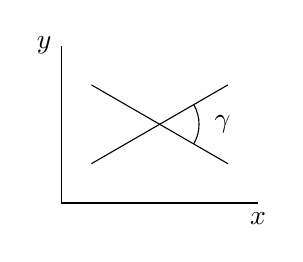
\begin{tikzpicture}
\draw(0,0)--++(2.5,0)node[below]{$x$};
\draw(0,0)--++(0,2)node[left]{$y$};
\draw(1.25,1)++(180-30:1)--++(-30:2);
\draw(1.25,1)++(-180+30:1)--++(30:2);
\draw([shift={(-30:0.5)}]1.25,1) arc (-30:30:0.5);
\draw(1.25,1)++(0.8,0)node[]{$\gamma$};
\end{tikzpicture}
\caption{ خوش خو نظام}
\end{subfigure} \hfill
\begin{subfigure}{0.45\textwidth}
\centering
\begin{tikzpicture}
\draw(0,0)--++(2.5,0)node[below]{$x$};
\draw(0,0)--++(0,2)node[left]{$y$};
\draw(1.25,1)++(-180+30:1)--++(30:2);
\draw(1.25,1)++(-180+35:1)--++(35:2);
\end{tikzpicture}
\caption{ بد خو نظام}
\end{subfigure} \hfill
\caption{دو متغیرات کے دو خطی مساوات کے نظام}
\label{شکل_خطی_اعدادی_بد_خو_خوش_خو}
\end{figure}

%==================
\ابتدا{مثال}\شناخت{مثال_اعدادی_خطی_بد_خو_الف}\quad \موٹا{بد خو نظام}\\
درج ذیل نظام
\begin{align*}
0.9999x-1.0001y&=1\\
x\phantom{1.0000}-y&=1
\end{align*}
کا حل \عددی{x=0.5}، \عددی{y=-0.5} ہے جبکہ نظام
\begin{align*}
0.9999x-1.0001y&=1\\
x\phantom{1.0000}-y&=1+\epsilon
\end{align*}
کا حل \عددی{x=0.5+5000.5\epsilon}، \عددی{y=-0.5+4999.5\epsilon} ہے۔آپ دیکھ سکتے ہیں کہ نظام بد خو ہے۔دائیں ہاتھ میں \عددی{\epsilon} تبدیلی سے نتائج میں تخمیناً  \عددی{5000\epsilon} تبدیلی پیدا ہوتی ہے۔
\انتہا{مثال}
%================================

ندرت تک پہنچنے کے عمل کو بد خوئی تصور کیا جا سکتا ہے۔دوران حساب ملحوظ ہندسوں کے کھوئے جانے سے بد خوئی عیاں ہوتی ہے۔یوں درست منعکس یا حل کا حصول زیادہ دشوار ثابت ہوتا ہے۔

بد خوئی کی صورت میں (اگر پور و پور خلل پایا جاتا ہو تب) کسی مقررہ اعشاریہ تک درست نتائج حاصل کرنے کی خاطر حساب میں نسبتاً بہت زیادہ اعشاریہ تک اعداد استعمال کرنے ہوں گے۔اگر بد خو نظام کا دایاں ہاتھ اور  عددی سر کسی کلیہ سے حاصل کیے جا سکتے ہوں تب ہم انہیں جتنی درستگی تک  چاہیں حاصل کر سکتے ہیں لہٰذا بد خوئی کا مسئلہ اتنا سنگین نہیں ہو گا۔اس کے برعکس اگر نظام کا دایاں ہاتھ اور اس کے عددی سر تجربہ سے حاصل کیے گئے ہوں تب (چونکہ کسی حد سے بہتر تجرباتی نتائج حاصل کرنا ممکن نہیں ہوتا ہے لہٰذا)   ان میں خلل کی گنجائش کو رد نہیں کیا جا سکتا ہے  اور صورت حال زیادہ سنگین ہو گی۔ہمیں ماننا  ہو گا کہ نظام کے مواد میں خلل کی بنا، بد خو نظام کے حل میں بہت زیادہ خلل پایا جائے گا۔ایسی صورت میں بہتر ہو گا کہ ہم نظام کو کسی ایسی مساواتوں سے ظاہر کریں جو نسبتاً زیادہ خوش خو ہوں۔

بد خوئی کی چند علامتیں کچھ یوں ہیں۔نظام کے دائیں ہاتھ اجزاء اور زیادہ سے زیادہ \عددی{\abs{a_{jk}}} کے لحاظ سے \عددی{\abs{\bM{A}\,\text{مقطع}}} چھوٹا ہو گا۔ کم درست تخمینی حل بہت کم  بقیہ پیدا کرتا ہو گا (نیچے دیکھیں)۔حل کے اجزاء کی مطلق قیمتوں کی نسبت \عددی{\bM{A}^{-1}} کے اجزاء کی مطلق قیمتیں بڑی ہوں گی۔ 

مرکزی وتر کے اجزاء کی مطلق قیمت باقی اجزاء کی مطلق قیمت سے زیادہ ہونے کی صورت میں خوش خو نظام پایا جائے گا۔اگر چکور قالب جس کے بڑے اجزاء \عددی{0.1} اور \عددی{10} کے بیچ ہوں کے معکوس کے بڑے اجزاء بھی لگ بھگ انہیں حدود میں پائے جاتے ہوں تب ان سے منسلک مساوات کا نظام خوش خو ہو گا۔ 

بد خوئی کی صورت میں ہم
\begin{align}\label{مساوات_خطی_اعدادی_نظام_بقیہ_الف}
\bM{A}\bM{x}=\bM{b}
\end{align}
کے تخمینی حل \عددی{\bM{x}_{(1)}} سے  بہتر حل تلاش کرنا چاہیں گے۔ \عددی{\bM{x}_{(1)}} کے لحاظ سے اس نظام کا مطابقتی \اصطلاح{بقیہ}\فرہنگ{بقیہ}\فرہنگ{residual} درج ذیل ہے۔ 
\begin{align*}
\bM{r}_{(1)}=\bM{b}-\bM{A}\bM{x}_{(1)}
\end{align*}
یوں 
\begin{align*}
\bM{A}\bM{x}_{(1)}=\bM{b}-\bM{r}_{(1)}
\end{align*}
لہٰذا
\begin{align}\label{مساوات_خطی_اعدادی_نظام_بقیہ_ب}
\bM{A}(\bM{x}-\bM{x}_{(1)})=\bM{r}_{(1)}
\end{align}
ہو گا۔اس سے ظاہر ہے کہ مساوات \حوالہ{مساوات_خطی_اعدادی_نظام_بقیہ_ب} کے حل کو بطور \عددی{\bM{r}_{(1)}}  کی درستگی استعمال کرتے ہوئے مساوات \حوالہ{مساوات_خطی_اعدادی_نظام_بقیہ_الف} کا حل حاصل ہو گا۔جب تک نظام بہت زیادہ بد خو نہ ہو، \عددی{\bM{r}_{(1)}} کے اجزاء \عددی{\bM{b}} کے اجزاء سے کم ہوں گے۔

%=======================
\حصہء{سوالات}

%==============
\ابتدا{سوال}\quad
مثال \حوالہ{مثال_اعدادی_خطی_بد_خو_الف} میں نظام کو سب سے بڑی مطلق قیمت والے عددی سر سے تقسیم کرتے ہوئے حاصل نظام کے قالب کا مقطع حاصل کریں۔تبصرہ کریں۔ کیا بد خو نظام کے قالب کے مقطع کی قیمت بڑی ہو سکتی ہے؟\\
جواب:\quad
$-0.0002$
\انتہا{سوال}
%====================
\ابتدا{سوال}\quad
\عددی{\xi=x+y+1} اور \عددی{\eta=x-y-1} پر کرتے ہوئے مثال \حوالہ{مثال_اعدادی_خطی_بد_خو_الف} سے دوسرا بد خو نظام حاصل کریں۔ 
\انتہا{سوال}
%=======================
\ابتدا{سوال}\شناخت{سوال_خطی_اعدادی_بد_خو_زاویہ_الف}\quad
درج ذیل دونوں نظام کو حل کریں۔ان کے حل کا آپس میں موازنہ کریں۔نتائج پر تبصرہ کریں۔
\begin{gather*}
\begin{aligned}
2x+1.4y&=1.4\\
1.4x+y&=1
\end{aligned}\quad\quad
\begin{aligned}
2x+1.4y&=1.44\\
1.4x+y&=1
\end{aligned}
\end{gather*}
جواب:\quad
$x=0,y=1;\quad x=1,y=-0.4$
\انتہا{سوال}
%=====================
\ابتدا{سوال}\quad
درج ذیل دونوں نظام کو حل کریں۔ان حل کا آپس میں موازنہ کریں۔نتائج پر تبصرہ کریں۔
\begin{gather*}
\begin{aligned}
5x-7y&=-2\\
-7x+10y&=\phantom{-}3
\end{aligned}\quad\quad
\begin{aligned}
5x-7y&=-2\\
-7x+10y&=\phantom{-}3.1
\end{aligned}
\end{gather*}
\انتہا{سوال}
%=====================
\ابتدا{سوال}\شناخت{سوال_خطی_اعدادی_بد_خو_زاویہ_ب}\quad
دکھائیں کہ دو لکیروں
\begin{align*}
a_{11}x_1+a_{12}x_2&=b_1\\
a_{21}x_1+a_{22}x_2&=b_2
\end{align*}
کے مابین زاویہ \عددی{\gamma} درج ذیل تعلق دیتا ہے۔
\begin{align*}
\tan \gamma=\frac{a_{11}a_{22}-a_{12}a_{21}}{a_{11}a_{21}+a_{12}a_{22}}
\end{align*}
بد خوئی کے نقطہ سے اس کلیہ پر تبصرہ کریں۔
\انتہا{سوال}
%====================
\ابتدا{سوال}\quad
مثال \حوالہ{مثال_اعدادی_خطی_بد_خو_الف} اور سوال \حوالہ{سوال_خطی_اعدادی_بد_خو_زاویہ_الف} کے نظام کے لئے زاویہ \عددی{\gamma} سوال \حوالہ{سوال_خطی_اعدادی_بد_خو_زاویہ_ب} کی مدد سے حاصل کریں۔نتائج پر تبصرہ کریں۔
\انتہا{سوال}
%====================
\ابتدا{سوال}\quad
دکھائیں کہ درج ذیل نظام کا حل \عددی{x_1=1}، \عددی{x_2=1}، \عددی{x_3=1} ہے۔
\begin{align*}
6x_1+7x_2+8x_3&=21\\
7x_1+8x_2+9x_3&=24\\
8x_1+9x_2+9x_3&=26
\end{align*}
نظام کا مقطع تلاش کریں اور \عددی{x_1=-0.8}، \عددی{x_2=2.9}، \عددی{x_3=0.7} کے لحاظ سے نظام کا بقیہ حاصل کریں۔\\
جواب:\quad
$1;\quad -0.1,0.1,0$
\انتہا{سوال}
%=========================
\ابتدا{سوال}\quad
دکھائیں کہ
\begin{align*}
\bM{A}=\begin{bmatrix}1.00&1.00\\1.00&1.01  \end{bmatrix}\quad\quad
\bM{B}=\begin{bmatrix*}[r]111&-100\\-110&100  \end{bmatrix*}
\end{align*}
کا \عددی{\bM{A}\bM{B}} تقریباً اکائی قالب کے برابر ہے جبکہ \عددی{\bM{B}\bM{A}} ایسا نہیں ہے۔تبصرہ کریں۔
\انتہا{سوال}
%==========================
\ابتدا{سوال}\quad \موٹا{(قالب ہلبرٹ)}  \quad 
گاوسی اسقاط سے نظام
\begin{align*}
x+\tfrac{1}{2}y+\tfrac{1}{3}z&=1\\
\tfrac{1}{2}x+\tfrac{1}{3}y+\tfrac{1}{4}z&=0\\
\tfrac{1}{3}x+\tfrac{1}{4}y+\tfrac{1}{5}z&=0
\end{align*}
کا حل \عددی{x=9}، \عددی{y=-36}، \عددی{z=30} تلاش کریں۔اب ایک وقت میں صرف دو ملحوظ ہندسے استعمال کرتے ہوئے اس نظام کو دوبارہ حل کریں۔نتائج کا موازنہ کریں اور ان پر تبصرہ کریں۔(اس نظام کے عددی سر قالب کو \عددی{3\times 3}  \اصطلاح{قالب ہلبرٹ}\فرہنگ{قالب!ہلبرٹ} کہتے ہیں۔)\\
جواب:\quad
پہلی قدم میں \عددی{0.08y+0.09z=-0.50}، \عددی{0.08y+0.09z=-0.33} حاصل ہو گا جہاں \عددی{0.165} کو دو ملحوظ ہندسوں میں عمومی قاعدہ کے تحت \عددی{0.16} لکھا گیا ہے۔دوسری قدم میں \عددی{0=0.17} حاصل ہو گا جو کوئی معنی نہیں رکھتا ہے۔اگر ہم \عددی{0.165} کو \عددی{0.17} لکھیں تب \عددی{z=17}، \عددی{y=-23}، \عددی{x=7.0} حاصل ہو گا۔نظام بد خو ہے۔
\انتہا{سوال}
%===================
\ابتدا{سوال}\quad 
تعریف کی رو سے \عددی{n\times n} قالب ہلبرٹ \عددی{\bM{H}_n=[h_{jk}]}  کے اجزاء \عددی{h_{jk}=\tfrac{1}{j+k-1}} ہوں گے۔\عددی{n} بڑھانے سے معکوس \عددی{\bM{H}_n^{-1}} کے اجزاء کی مطلق قیمتیں بہت زیادہ شرح سے بڑھتی ہیں۔اس حقیقت کو دیکھنے کی خاطر \عددی{\bM{H}_2^{-1}}، \عددی{\bM{H}_3^{-1}}،\عددی{\bM{H}_4^{-1}} تلاش کریں۔
\انتہا{سوال}
%====================

\حصہ{ترکیب کمتر مربع}
دیے گئے \عددی{n} عدد نقطوں (عددی جوڑیاں)
\begin{align*}
(x_1,y_1),\cdots,(x_n,y_n)
\end{align*}
پر \موٹا{منحنی بٹھانا}\فرہنگ{منحنی بٹھانا}\حاشیہب{curve fitting}\فرہنگ{curve fitting}  سے مراد ایسے تفاعل \عددی{f(x)} کی تلاش ہے  جو  \عددی{j=1,\cdots,n} کے لئے \عددی{f(x_j)\approx y_j} پر پورا اترتا ہو۔اس عمل میں دیے گئے نقطوں کے لحاظ سے موافق منحنی تلاش کی جاتی ہے لہٰذا اس  کو  \اصطلاح{موافقت منحنی}\فرہنگ{موافقت منحنی} بھی کہتے ہیں۔تفاعل کی قسم (مثلاً کثیر رکنی، قوت نمائی تفاعل، سائن تفاعل، کوسائن تفاعل) کے بارے میں معلومات مسئلے کی نوعیت (یعنی طبعی وجوہات) سے حاصل کی جا سکتی ہے۔عموماً صورتوں میں کسی مخصوص درجے کی کثیر رکنی سے  موزوں منحنی حاصل کرنا ممکن ہو گا۔

 اگر ہمیں  سختی سے  مکمل برابری  \عددی{f(x_1)=y_1,\cdots,f(x_n)=y_n} درکار ہو تب باہمی تحریف کے کلیات استعمال کرتے ہوئے  ہم کافی زیادہ درجے کی کثیر رکنی \عددی{f(x)} حاصل کر سکتے ہیں۔البتہ کئی بار ایسا کرنے سے  قابل قبول نتائج حاصل نہیں ہوتے ہیں۔مثال کے طور پر ان تراکیب کو استعمال کرتے ہوئے درج ذیل چار نقطوں
\begin{align}\label{مساوات_خطی_اعدادی_کمتر_مربع_شرائط_الف}
(-1.0,1.000),\quad (-0.1,1.099),\quad (0.2,0.808),\quad (1.0,1.000)
\end{align}
سے گزرتی لیگرینج کثیر رکنی \عددی{f(x)=x^3-x+1} تلاش کی جا سکتی ہے جس کو شکل \حوالہ{شکل_اعدادی_خطی_تلاش_موزوں_منحنی}-الف میں دکھایا گیا ہے۔البتہ شکل \حوالہ{شکل_اعدادی_خطی_تلاش_موزوں_منحنی}-ب کو دیکھ کر صاف ظاہر ہوتا ہے کہ یہ نقطے تقریباً ایک سیدھی لکیر پر پائے جاتے ہیں۔اگر یہ نقطے کسی تجربہ سے حاصل کیے گئے ہوں تب ظاہر ہے کہ ان نقطوں میں خلل پایا جائے گا اور سیدھی لکیر پر پائے جانے والے نقطے اسی  (شکل) طرح دکھائی دیں گے۔اب اگر تجربے کی طبیعیات کہتی ہے کہ نتائج سیدھی لکیر پر آنے چاہیے تب ہم سیدھی لکیر کو درست تصور کریں گے۔ایسی موزوں (حاصل کردہ) منحنی سے کسی دوسری \عددی{x} کے لئے بھی قیمتیں اخذ کی جا سکتی ہیں۔عموماً صورتوں میں آنکھ سے دیکھ کر موزوں سیدھی لکیر تلاش کی جا سکتی ہے البتہ بہت زیادہ بکھرے  ہوئے نقطوں کی صورت میں ایسا کرنا قابل اعتماد نہیں ہو گا اور حسابی تراکیب استعمال کرنا بہتر ہو گا۔ایسی ایک اہم ترکیب جو گاوس نے پیش کی  \اصطلاح{ترکیب کمتر مربع}\فرہنگ{ترکیب!کمتر مربع}\فرہنگ{کمتر مربع!ترکیب}\حاشیہب{method of least squares}\فرہنگ{least squares!method of} کہلاتی ہے۔
\begin{figure}
\centering
\begin{subfigure}{0.45\textwidth}
\centering
\begin{tikzpicture}
\draw(-1.5,0)--(1.5,0)node[right]{$x$};
\draw(0,0)--(0,2)node[left]{$y$};
\draw(-1,1)node[circ]{} (-0.1,1.099)node[circ]{} (0.2,0.808)node[circ]{} (1,1)node[circ]{};
\draw[thick,domain=-1.3:1.3] plot ({\x},{\x^3-\x+1});
\foreach \x in {-1,0,1}{\draw(\x,0)node[below]{$\x$}--++(0,0.1);}
\end{tikzpicture}
\caption{ چار نقطوں سے گزرتی ہوئی کثیر رکنی}
\end{subfigure} \hfill
\begin{subfigure}{0.45\textwidth}
\centering
\begin{tikzpicture}
\draw(-1.5,0)--(1.5,0)node[right]{$x$};
\draw(0,0)node[below]{$0$}--(0,2)node[left]{$y$};
\draw(-1,1)node[circ]{} (-0.1,1.099)node[circ]{} (0.2,0.808)node[circ]{} (1,1)node[circ]{};
\draw[thick,domain=-1.5:1.5] plot ({\x},{0.9773-0.0224*\x});
\foreach \x in {-1,1}{\draw(\x,0)node[below]{$\x$}--++(0,0.1);}
\draw(0,0.5)node[left]{$0.5$}--++(0.1,0);
\draw(0,1)node[above right]{$1$};
\end{tikzpicture}
\caption{ چار نقطوں سے گزرتی ہوئی سیدھی لکیر}
\end{subfigure} \hfill
\caption{تلاش موافق منحنی}
\label{شکل_اعدادی_خطی_تلاش_موزوں_منحنی}
\end{figure} 

\جزوحصہء{ترکیب کمتر مربع}
ہمیں سیدھی لکیر
\begin{align*}
y=a+bx
\end{align*}
کو نقطوں \عددی{(x_1,y_1),\cdots,(x_n,y_n)} کے بیچ یوں رکھنا ہے کہ نقطوں سے لکیر تک فاصلوں کے مربع کا مجموعہ کم سے کم ہو جہاں فاصلہ عمودی رخ (\عددی{y} کے متوازی) ناپا جاتا ہے۔
\begin{figure}
\centering
\begin{tikzpicture}
\draw(0,2.5)node[left]{$y$}--(0,0)--(5,0)node[below]{$x$};
\draw(0.25,0.5)--(3.75,1.5)coordinate[pos=0.75](kA)node[pos=1,right]{$y=a+bx$};
\draw(kA)++(0,1)coordinate(kT)node[circ]{}node[right]{$(x_j,y_j)$}--($(0,0)!(kA)!(4,0)$)node[below]{$x_j$};
\draw(kA)node[ocirc]{};
\draw(kT)++(-0.25,0)--++(-0.25,0)coordinate[pos=0.5](kTT);
\draw(kA)++(-0.25,0)--++(-0.25,0)coordinate[pos=0.5](kAA);
\draw[stealth-stealth] (kTT)--(kAA)node[pos=0.5,left]{$y_j-a-bx_j$};
\draw(kA)++(0.25,0)--++(0.25,0)coordinate[pos=0.5](kAA);
\draw[stealth-stealth] (kAA)--($(0,0)!(kAA)!(4,0)$)node[pos=0.5,right]{$a+bx_j$};
\end{tikzpicture}
\caption{نقطہ کا لکیر سے انتصابی فاصلہ}
\label{شکل_خطی_اعدادی_انتصابی_فاصلہ}
\end{figure}

شکل \حوالہ{شکل_خطی_اعدادی_انتصابی_فاصلہ} میں نقطہ \عددی{(x_j,y_j)} اور لکیر \عددی{y=a+bx} دکھائے گئے ہیں۔\عددی{(x_j,0)} سے لکیر تک انتصابی فاصلہ \عددی{a+bx_j} ہے۔یوں \عددی{(x_j,y_j)} سے لکیر تک انتصابی فاصلہ \عددی{\abs{y_j-a-bx_j}} ہو گا۔یوں تمام دیے گئے نقطوں کا لکیر سے انتصابی فاصلوں کے مربع کا مجموعہ
\begin{align*}
q=\sum_{j=1}^{n} (y_j-a-bx_j)^2
\end{align*}
ہو گا جہاں \عددی{q} کی قیمت \عددی{a} اور \عددی{b} کے تابع ہو گی۔\عددی{q} کی کم سے کم قیمت تلاش کرنے کے شرائط درج ذیل ہیں (جہاں ہم \عددی{j=1} تا \عددی{j=n} مجموعہ لیتے ہیں۔)
\begin{gather}
\begin{aligned}\label{مساوات_خطی_اعدادی_کمتر_مربع_شرائط_ب}
\frac{\partial q}{\partial a}&=-2\sum(y_j-a-bx_j)=0\\[0.5ex]
\frac{\partial q}{\partial b}&=-2\sum x_j(y_j-a-bx_j)=0
\end{aligned} 
\end{gather}
یوں 
\begin{gather}
\begin{aligned}\label{مساوات_خطی_اعدادی_کمتر_مربع_شرائط_پ}
an+b\sum x_j&=\sum y_j\\[0.5ex]
a\sum x_j+b\sum x_j^2&=\sum x_jy_j
\end{aligned}
\end{gather}
حاصل ہوتے ہیں جنہیں ہمارے مسئلے کی \اصطلاح{عمودی مساوات}\فرہنگ{کمتر مربع!عمودی مساوات}\حاشیہب{normal equations}\فرہنگ{least squares!normal equations} کہتے ہیں۔

%=====================
\ابتدا{مثال}\quad \موٹا{سیدھی لکیر}\\
ترکیب کمتر مربع استعمال کرتے ہوئے  مساوات \حوالہ{مساوات_خطی_اعدادی_کمتر_مربع_شرائط_الف} میں دیے گیے چار نقطوں پر  سیدھی لکیر بٹھائیں۔\\
حل:\quad یہاں
\begin{align*}
n=4,\quad \sum x_j=0.1,\quad \sum x_j^2=2.05,\quad \sum y_j=3.907, \quad \sum x_jy_j=0.0517
\end{align*}  
ہیں لہٰذا عمودی مساوات
\begin{align*}
4a+0.10b&=3.9070\\
0.1a+2.05b&=0.0517
\end{align*}
ہوں گے جن کا حل \عددی{a=0.9773}، \عددی{b=-0.0224} ہے۔یوں درج ذیل سیدھی لکیر (شکل \حوالہ{شکل_اعدادی_خطی_تلاش_موزوں_منحنی}-ب) حاصل ہو گی۔
\begin{align*}
y=0.9773-0.0224x
\end{align*}
\انتہا{مثال}
%============================

ہم نقطوں پر سیدھی لکیر \عددی{y=a+bx} کی بجائے درجہ \عددی{m} کی موزوں کثیر رکنی
\begin{align*}
p(x)=b_0+b_1x+\cdots+b_mx^m
\end{align*}
بٹھا سکتے ہیں جہاں \عددی{m\le n-1} ہے۔تب \عددی{q} کی صورت 
\begin{align*}
q=\sum_{j=1}^{n}(y_j-p(x_j))^2
\end{align*}
ہو گی جو \عددی{m+1} عدد متغیر معلوم \عددی{b_0,\cdots,b_m} کا تابع ہے۔اب مساوات \حوالہ{مساوات_خطی_اعدادی_کمتر_مربع_شرائط_ب} کی  جگہ ہمارے پاس درج ذیل \عددی{m+1} شرائط ہوں گے
\begin{align*}
\frac{\partial q}{\partial b_0}=0,\cdots,\frac{\partial q}{\partial b_m}=0
\end{align*}
جو \عددی{m+1}  عمودی مساوات کا نظام ہے۔دو درجی کثیر رکنی
\begin{align}\label{مساوات_خطی_اعدادی_کمتر_مربع_شرائط_ت}
p(x)=b_0+b_1x+b_2x^2
\end{align}
 کی صورت میں آپ تسلی کر لیں کہ عمودی مساوات (\عددی{1} تا \عددی{n} کا مجموعہ)
\begin{gather}
\begin{aligned}\label{مساوات_خطی_اعدادی_کمتر_مربع_شرائط_ٹ}
b_0 n\phantom{\sum {}_j}+b_1\sum x_j+b_2\sum x_j^2&=\sum y_j\\[0.5ex]
b_0 \sum x_j +b_1\sum x_j^2 +b_2\sum x_j^3&=\sum x_jy_j\\[0.5ex]
b_0 \sum x_j^2+b_1\sum x_j^3+b_2\sum x_j^4&=\sum x_j^2y_j
\end{aligned}
\end{gather}
ہو گا۔ آپ دیکھ سکتے ہیں کہ یہ نظام تشاکلی ہے۔حصہ \حوالہ{حصہ_خطی_اعدادی_گاوس_اسقاط_معکوس_قالب} اور حصہ \حوالہ{حصہ_خطی_اعدادی_حل_بذریعہ_اعادہ} میں دی گئی تراکیب سے اس نظام کو حل کیا جا سکتا ہے۔

%==============================

\حصہء{سوالات}
سوال \حوالہ{سوال_خطی_اعدادی_کمتر_مربع_الف} تا سوال \حوالہ{سوال_خطی_اعدادی_کمتر_مربع_ب} میں دیے گئے نقطوں پر سیدھی لکیر (الف) آنکھ سے دیکھ کر، (ب)  ترکیب کمتر مربع استعمال کرتے ہوئے  بٹھائیں۔ 

%================
\ابتدا{سوال}\شناخت{سوال_خطی_اعدادی_کمتر_مربع_الف}\quad
$(5,10.0), (10,8.9), (15,8.2), (20,7.0)$\\
جواب:\quad
$y=10.96-0.194x$

\انتہا{سوال}
%======================
\ابتدا{سوال}\quad
$(0,0),(1,1.1), (2,1.9), (3,3.1)$\\
جواب:\quad
$y=0.01+1.01x$
\انتہا{سوال}
%======================
\ابتدا{سوال}\quad
$(4,-17), (15,-4), (30,-7), (100,50), (200,70)$\\
جواب:\quad
$y=-13.503+0.457x$
\انتہا{سوال}
%======================
\ابتدا{سوال}\quad
$(2,0), (3,4), (4,10), (5,16)$\\
جواب:\quad
$y=-11.4+5.4x$
\انتہا{سوال}
%======================
\ابتدا{سوال}\quad
\begin{align*}
\centering
%\begin{otherlanguage}{english}
\begin{array}{CCCCCCCCCLR}
2.8&2.9&3.0&3.1&3.2&3.2&3.2&3.3&3.4&$x\,[\si{\gram \per\centi\meter\cubed}]$&\text{\RL{{خام دھات}}}\\
30&26&33&31&33&35&37&36&33&$y\,[\si{\percent}]$&\text{\RL{{لوہا کی مقدار}}}
\end{array}
%\end{otherlanguage}
\end{align*}
جواب:\quad
$y=-5.05+12.1x$
\انتہا{سوال}
%==============================
\ابتدا{سوال}\quad
\begin{align*}
\centering
%\begin{otherlanguage}{english}
\begin{array}{CCCCCLR}
400&500&600&700&750&$x$&\text{\RL{{فی منٹ چکر}}}\\
580&1030&1420&1880&2100&$y\,[\si{\kilo\watt}]$&\text{\RL{{انجن کی طاقت}}}
\end{array}
%\end{otherlanguage}
\end{align*}
\انتہا{سوال}
%==============================
\ابتدا{سوال}\شناخت{سوال_خطی_اعدادی_کمتر_مربع_ب}\quad
سیدھی سڑک پر  ایک گاڑی مستقل رفتار \عددی{v=b_1 \,\si{\meter\per\second}} سے چلتے ہوئے وقت  \عددی{t\,[\si{\second}]} میں \عددی{y=b_0+b_1t} فاصلہ طے کرے گی۔مختلف لمحات پر درج ذیل فاصلے ناپے جاتے ہیں۔
\begin{align*}
\centering
%\begin{otherlanguage}{english}
\begin{array}{CCCCCLR}
0&3&5&8&10&$t\,[\si{\second}]$&\text{\RL{{وقت}}}\\
100&130&140&170&190&$y\,[\si{\meter}]$&\text{\RL{{فاصلہ}}}
\end{array}
%\end{otherlanguage}
\end{align*}
ان نقطوں کو \عددی{ty} سطح پر کھینچیں۔ان نقطوں پر سیدھی لکیر (الف) آنکھ سے دیکھتے ہوئے، (ب) ترکیب کمتر مربع کی استعمال سے بٹھائیں۔اس سیدھی لکیر سے رفتار کی تخمینی قیمت حاصل کریں۔\\
جواب:\quad
$y=100.127+8.822t, \quad v=\SI{8.822}{\meter\per\second}$
\انتہا{سوال}
%==================================
سوال \حوالہ{سوال_خطی_اعدادی_موزوں_قطع_مکافی_الف} تا سوال \حوالہ{سوال_خطی_اعدادی_موزوں_قطع_مکافی_ب} میں ترکیب کمتر مربع کی مدد سے مساوات \حوالہ{مساوات_خطی_اعدادی_کمتر_مربع_شرائط_ت} استعمال کرتے ہوئے  نقطوں پر قطع مکافی بٹھائیں۔

%==========================
\ابتدا{سوال}\شناخت{سوال_خطی_اعدادی_موزوں_قطع_مکافی_الف}\quad
$(0,3),(1,1),(2,0),(4,1),(6,4)$
\انتہا{سوال}
%=========================
\ابتدا{سوال}\شناخت{سوال_خطی_اعدادی_درکار_موزوں_قطع_مکافی_الف}\quad
$(-1,0),(0,-2),(0,-1),(1,0)$\\
جواب:\quad
$y=-1.5+1.5x^2$
\انتہا{سوال}
%======================
\ابتدا{سوال}\quad
$(1.09,1.35),(1.28,1.58),(1.36,1.68),(1.44,1.85),(1.60,2.23),(1.65,2.38)$

\انتہا{سوال}
%======================
\ابتدا{سوال}\quad
معمولی ڈھلوان پر چلتے ہوئے ٹریکٹر کی رفتار بالمقابل بوجھ دیا گیا ہے۔
\begin{align*}
\centering
%\begin{otherlanguage}{english}
\begin{array}{CCCCCLR}
1.4&1.8&2.3&3.0&4.0&$x\,[\si{\kilo\meter\per\hour}]$&\text{\RL{{رفتار}}}\\
7400&7500&7600&7500&7200&$y\,[\si{\kilogram}]$&\text{\RL{{کمیت}}}
\end{array}
%\end{otherlanguage}
\end{align*}
جواب:\quad
$y=6642+762.3x-156.1x^2$
\انتہا{سوال}
%==============================
\ابتدا{سوال}\شناخت{سوال_خطی_اعدادی_موزوں_قطع_مکافی_ب}\quad
\begin{align*}
\centering
%\begin{otherlanguage}{english}
\begin{array}{CCCCCCLR}
1&2&3&4&5&6&$x\,[\si{\hour}]$&\text{\RL{{مزدور کا کام کرنے کا دورانیہ}}}\\
1.50&1.48&1.75&1.65&1.72&1.55&$y\,[\si{\second}]$&\text{\RL{{رد عمل میں دیری}}}
\end{array}
%\end{otherlanguage}
\end{align*}
\انتہا{سوال}
%==============================
\ابتدا{سوال}\quad
ترکیب شولسکی سے سوال \حوالہ{سوال_خطی_اعدادی_درکار_موزوں_قطع_مکافی_الف} کو حل کریں۔
\انتہا{سوال}
%=============================
\ابتدا{سوال}\quad
تین درجی کثیر رکنی کی صورت میں عمودی مساوات حاصل کریں۔
\انتہا{سوال}
%=======================
\ابتدا{سوال}\quad
ہم ترکیب کمتر مربع میں کثیر رکنی
\begin{align*}
b_0+b_1x_j+b_2x_j^2+\cdots,+b_mx_j^m=y_j,\quad \quad (j=1,\cdots,n)
\end{align*}
کو مطمئن کرنے کی کوشش کرتے ہیں۔ایسا قالب \عددی{\bM{C}} متعارف کریں کہ اس کثیر رکنی کو ہم \عددی{\bM{C}\bM{b}=\bM{y}} لکھ سکیں۔دکھائیں کہ تب عمودی مساوات \عددی{\bM{C}^T\bM{C}\bM{b}=\bM{C}^T\bM{y}} لکھے جا سکتے ہیں۔ \\
جواب:\quad
$\bM{C}=[c_{jk}],\, c_{jk}=x_j^{k-1},\, \bM{b}^T=[b_0\cdots b_m]$
\انتہا{سوال}
%========================
\ابتدا{سوال}\quad
نمو آبادی کے مسئلہ میں عموماً موزوں قوت نمائی تفاعل \عددی{y=b_0e^{bx}} کو ترکیب کمتر مربع  کی استعمال سے حاصل کرنا ہو گا۔دکھائیں کہ دونوں ہاتھ لوگارتھم لے کر اس مسئلہ کو   سیدھی لکیر بٹھانے  کے مسئلہ میں تبدیل کیا جا سکتا ہے۔\\
جواب:\quad
$y^*=a^*+bx,\quad y^*=\ln y,\, a^*=\ln b_0$ 
\انتہا{سوال}
%============================

\حصہ{قالب کے امتیازی اقدار کی شمول}
\عددی{n} صف پر مشتمل (حقیقی یا مخلوط) چکور قالب \عددی{\bM{A}=[a_{jk}]} کے  \اصطلاح{امتیازی اقدار}\فرہنگ{امتیازی!اقدار}  یا \اصطلاح{آئگنی اقدار}\فرہنگ{آئگنی!اقدار} سے مراد ایسا عدد \عددی{\lambda} ہے جس کے لئے
\begin{align}\label{مساوات_خطی_اعدادی_گرشگرین_الف}
\bM{A}\bM{x}=\lambda \bM{x}
\end{align}
کا غیر صفر حل یعنی \عددی{\bM{x}\ne \bM{0}} پایا جاتا ہو جو اس \عددی{\lambda} کے لحاظ سے \عددی{\bM{A}} کا \اصطلاح{امتیازی سمتیہ}\فرہنگ{امتیازی!سمتیہ} یا \اصطلاح{آئگنی سمتیہ}\فرہنگ{آئگنی!سمتیہ} کہلاتا ہے۔\عددی{\bM{A}} کے تمام امتیازی اقدار کے سلسلہ کو \عددی{\bM{A}} کا \اصطلاح{طیف}\فرہنگ{طیف} کہتے ہیں۔\عددی{\bM{A}} کے امتیازی اقدار درج ذیل امتیازی مساوات
\begin{align}\label{مساوات_خطی_اعدادی_گرشگرین_ب}
D(\lambda)=(\bM{A}-\lambda \bM{I})\, \text{مقطع} =0
\end{align}
کے جذر ہوں گے جہاں  \عددی{\bM{I}} اکائی قالب ہے جو  \عددی{n} صف پر مشتمل ہے۔\عددی{D(\lambda)} کو \اصطلاح{امتیازی مقطع}\فرہنگ{امتیازی!مقطع} کہتے ہیں جس کو \عددی{\lambda} کے \عددی{n} درجی کثیر رکنی کی صورت میں  لکھا جا سکتا ہے جو \عددی{\bM{A}} کا مطابقتی \اصطلاح{امتیازی کثیر رکنی}\فرہنگ{امتیازی!کثیر رکنی}  کہلاتا ہے۔یوں \عددی{\bM{A}} کا کم از کم ایک امتیازی قدر  اور زیادہ سے زیادہ \عددی{n} منفرد امتیازی اقدار ممکن ہوں گے۔

کسی بھی \عددی{\bM{A}} کے  امتیازی کثیر رکنی کے عددی سر حاصل کر کے کثیر رکنی کا جذر تلاش کیا جا سکتا ہے۔البتہ بڑی \عددی{n} کی صورت میں کثیر رکنی کے عددی سر تلاش کرنا اور کثیر رکنی کا جذر تلاش کرنا خاصہ لمبا کام ثابت ہو گا لہٰذا بہتری اسی میں ہے کہ کوئی بہتر ترکیب استعمال کی جائے۔ حقیقتاً ایسے دو قسم کے تراکیب پائے جاتے ہیں۔
\begin{itemize}
\item
امتیازی اقدار کے حدود تلاش کرنے کے تراکیب۔
\item
امتیازی اقدار کے تخمینی قیمتیں تلاش کرنے کے تراکیب۔
\end{itemize}

ہم دونوں ترکیب کو مثالوں کی مدد سے سمجھتے ہیں۔

درج ذیل دلچسپ \اصطلاح{مسئلہ گرشگرین}\فرہنگ{مسئلہ!گرشگرین}\حاشیہب{Gershgorin's theorem}\فرہنگ{theorem!Gershgorin} ایسی دائری اقراص پر مشتمل خطہ دیتا ہے جس میں دیے گئے قالب کے تمام امتیازی اقدار پائے جاتے ہیں۔درحقیقت ہر \عددی{k=1,\cdots,n} کے لئے اس مسئلہ\حاشیہد{روسی ریاضی دان سمیون ارانووچ گرشگرین [1901-1933]} میں دیا گیا عدم مساوات ایک دائری قرص کو ظاہر کرتی ہے جس کا مرکز، مخلوط \عددی{\lambda} سطح میں \عددی{a_{kk}} ہے اور جس کا رداس، عدم مساوات کا دایاں ہاتھ دیتا ہے؛ اور یہ مسئلہ کہتا ہے کہ \عددی{\bM{A}} کا ہر ایک امتیازی قدر ان \عددی{n} عدد اقراص میں سے کسی نا کسی  ایک میں پایا جائے گا۔

%======================
\ابتدا{مسئلہ}\شناخت{مسئلہ_خطی_اعدادی_گرشگرین}\quad \موٹا{(مسئلہ گرشگرین)}\\
فرض کریں کہ کسی \عددی{n\times n} قالب \عددی{\bM{A}=[a_{jk}]} کا امتیازی قدر \عددی{\lambda} ہے۔تب کسی عدد صحیح \عددی{k\, (1\le k\le n)} کے لئے درج ذیل ہو گا۔
\begin{align}\label{مساوات_خطی_اعدادی_گرشگرین_پ}
\abs{a_{kk}-\lambda}\le \abs{a_{k1}}+\abs{a_{k2}}+\cdots+\abs{a_{k,k-1}}+\abs{a_{k,k+1}}+\cdots+\abs{a_{kn}}
\end{align}
\انتہا{مسئلہ}
%=======================
\ابتدا{ثبوت}\quad
فرض کریں کہ \عددی{\bM{A}} کے اس امتیازی قدر \عددی{\lambda} کا مطابقتی امتیازی سمتیہ \عددی{\bM{x}} ہے۔تب
\begin{align}\label{مساوات_خطی_اعدادی_گرشگرین_ٹ}
\bM{A}\bM{x}=\lambda\bM{x}\quad \implies \quad (\bM{A}-\lambda \bM{I})\bM{x}=\bM{0}
\end{align}
ہو گا۔فرض کریں کہ \عددی{\bM{x}} کے اجزاء میں سب سے زیادہ مطلق قیمت والا جزو \عددی{x_k} ہے۔ تب
\begin{align*}
\tfrac{x_m}{x_k}\le 1\quad \quad \quad  (m=1,\cdots, n)
\end{align*}
ہو گا۔سمتی مساوات \حوالہ{مساوات_خطی_اعدادی_گرشگرین_ٹ} درحقیقت \عددی{n} مساوات کا نظام ہے جو مساوات کے دونوں اطراف سمتیات کے \عددی{n} اجزاء پر مشتمل ہے۔ان میں سے \عددی{k} ویں مساوات
\begin{align*}
a_{k1}x_1+\cdots+a_{k,k-1}x_{k-1}+(a_{kk}-\lambda)x_k+a_{k,k+1}x_{k+1}+\cdots+a_{kn}x_n=0
\end{align*}
ہو گی جس سے 
\begin{align*}
a_{kk}-\lambda=-a_{k1}\frac{x_1}{x_k}-\cdots-a_{k,k-1}\frac{x_{k-1}}{x_k}-a_{k,k+1}\frac{x_{k+1}}{x_k}-\cdots-a_{kn}\frac{x_{n}}{x_k}
\end{align*}
حاصل ہو گا۔اس کے دونوں اطراف مطلق قیمتیں لے کر تکونی عدم مساوات \عددی{\abs{a+b}\le \abs{a}+\abs{b}} (جہاں \عددی{a} اور \عددی{b} کوئی بھی مخلوط اعداد ہو سکتے ہیں) کی اطلاق سے اور
\begin{align*}
\abs{\frac{x_1}{x_k}}\le 1,\cdots, \quad \abs{\frac{x_n}{x_k}}\le 1
\end{align*}
 کو مد نظر رکھتے ہوئے  مساوات \حوالہ{مساوات_خطی_اعدادی_گرشگرین_پ} حاصل ہو گا۔یوں ثبوت مکمل ہوتا ہے۔
\انتہا{ثبوت}
%=========================

\ابتدا{مثال}\شناخت{مثال_خطی_اعدادی_گرشگرین_الف}\quad \موٹا{مسئلہ گرشگرین کا اطلاق}\\
قالب
\begin{align*}
\bM{A}=
\begin{bmatrix*}[r]26&-2&2\\ 2&21&4\\4&2&28  \end{bmatrix*}
\end{align*}
کے امتیازی اقدار مسئلہ \حوالہ{مسئلہ_خطی_اعدادی_گرشگرین} کے تحت  درج ذیل تین اقراص میں پائے جائیں گے (شکل \حوالہ{شکل_مثال_خطی_اعدادی_گرشگرین_الف})۔
\begin{itemize}
\item
\عددی{:D_1} رداس \عددی{\abs{-2}+2=4} اور مرکز \عددی{26}،
\item
\عددی{:D_2} رداس \عددی{2+4=6} اور مرکز \عددی{21}،
\item
\عددی{:D_3} رداس \عددی{4+2=6} اور مرکز \عددی{28}
\end{itemize}
آپ تسلی کر لیں کہ امتیازی اقدار \عددی{30}، \عددی{25} اور \عددی{20} ہیں۔
\begin{figure}
\centering
\begin{tikzpicture}[x={0.25cm},y={0.25cm}]
\draw(-10,0)--(17,0);
\draw(0,0)node[ocirc]{}node[below]{$21$} circle (6);
\draw(5,0)node[ocirc]{}node[below]{$26$} circle (4);
\draw(7,0)node[ocirc]{}node[below]{$28$} circle (6);
\draw(135:6)node[fill=white]{$D_2$};
\draw(5,0)++(45:4)node[fill=white]{$D_1$};
\draw(7,0)++(45:6)node[fill=white]{$D_3$};
\end{tikzpicture}
\caption{شکل برائے مثال \حوالہ{مثال_خطی_اعدادی_گرشگرین_الف}}
\label{شکل_مثال_خطی_اعدادی_گرشگرین_الف}
\end{figure}
\انتہا{مثال}
%=========================

امتیازی اقدار کی مطلق قیمتوں کا حد درج ذیل \اصطلاح{مسئلہ شُر}\فرہنگ{مسئلہ!شُر}\حاشیہب{Schur's theorem}\فرہنگ{theorem!Schur} دیتا ہے۔ مسئلہ شُر کا ثبوت اس کتاب میں پیش نہیں کیا جائے گا۔

\ابتدا{مسئلہ}\شناخت{مسئلہ_خطی_اعدادی_شر}\quad \موٹا{(مسئلہ شُر)}\حاشیہد{روسی ریاضی دان اسائے شُر [1875-1941]}\\
فرض کریں کہ \عددی{n\times n} قالب \عددی{\bM{A}=[a_{jk}]} کے امتیازی اقدار \عددی{\lambda_1,\cdots,\lambda_n} ہیں۔تب درج ذیل ہو گا۔
\begin{align}\label{مساوات_خطی_اعدادی_عدم_شر_الف}
\sum_{i=1}^{n}\abs{\lambda_i}^2\le \sum_{j=1}^{n}\sum_{k=1}^{n}\abs{a_{jk}}^2\quad \quad (\text{\RL{عدم مساوات شُر}})
\end{align}
مساوات \حوالہ{مساوات_خطی_اعدادی_عدم_شر_الف} میں  صرف اور صرف اس صورت برابری کا نشان استعمال ہو گا جب \عددی{\bM{A}} درج ذیل کو مطمئن کرتا ہو۔
\begin{align}\label{مساوات_خطی_اعدادی_عدم_شر_ب}
\bar{\bM{A}}^T\bM{A}=\bM{A}\bar{\bM{A}}^T
\end{align}
\انتہا{مسئلہ}
%=========================

مساوات \حوالہ{مساوات_خطی_اعدادی_عدم_شر_ب} کو مطمئن کرنے والا قالب \اصطلاح{عمودی}\فرہنگ{عمودی}\حاشیہب{normal}\فرہنگ{normal} کہلاتا ہے۔آپ دیکھ سکتے ہیں کہ ہرمشی، منحرف ہرمشی اور اکہرا قالب عمودی ہوں گے۔اسی طرح حقیقی تشاکلی، منحرف تشاکلی اور معیاری عمودی قالب بھی عمودی ہوں گے۔

فرض کریں کہ مسئلہ \حوالہ{مسئلہ_خطی_اعدادی_شر} میں قالب \عددی{\bM{A}} کا امتیازی قدر \عددی{\lambda_m} ہے تب \عددی{\abs{\lambda_m}^2} کی قیمت  مساوات \حوالہ{مساوات_خطی_اعدادی_عدم_شر_الف} کے بائیں ہاتھ کے برابر یا اس سے کم ہو گی لہٰذا دونوں اطراف جذر لیتے ہوئے
\begin{align}\label{مساوات_خطی_اعدادی_عدم_شر_پ}
\lambda_m\le \sqrt{ \sum_{j=1}^{n}\sum_{k=1}^{n}\abs{a_{jk}}^2}
\end{align}
حاصل ہو گا جس کے دائیں ہاتھ کو عموماً  \عددی{\bM{A}} کا \اصطلاح{معیار فروبنیوس}\فرہنگ{معیار!فروبنیوس}\حاشیہب{Frobenius norm}\فرہنگ{norm!Frobenius} یا \اصطلاح{معیار شُر}\فرہنگ{معیار!شُر}\حاشیہب{Schur norm}\فرہنگ{norm!Schur} کہتے ہیں۔ 

%===================
\ابتدا{مثال}\quad \موٹا{شُر عدم مساوات سے امتیازی اقدار کے حدود کا حصول}\\
مساوات \حوالہ{مساوات_خطی_اعدادی_عدم_شر_پ} سے مثال \حوالہ{مثال_خطی_اعدادی_گرشگرین_الف} کی قالب \عددی{\bM{A}} کے لئے درج ذیل حاصل ہو گا۔
\begin{align*}
\abs{\lambda}\le \sqrt{1949}<44.2
\end{align*}
(\عددی{\bM{A}} کے امتیازی اقدار \عددی{30}، \عددی{25}، \عددی{20} ہیں لہٰذا \عددی{30^2+25^2+20^2=1925<1949} ہے۔درحقیقت \عددی{\bM{A}} عمودی نہیں ہے۔)
\انتہا{مثال}
%==========================

مسئلہ گرشگرین اور مسئلہ شُر ہر حقیقی چکور قالب اور ہر مخلوط چکور قالب کے لئے درست ہیں۔کچھ مسئلے صرف مخصوص قسم کے قالب کے لئے درست ہوں گے۔درج ذیل \اصطلاح{مسئلہ پیغوں فروبنیوس}\فرہنگ{مسئلہ!پیغوں فروبنیوس}\حاشیہب{Perron-Frobenius's theorem}\فرہنگ{theorem!Perron-Frwbenius}،  جس کا ثبوت اس کتاب میں پیش نہیں کیا جائے گا، اسی نوعیت کا ہے۔ 

%====================
\ابتدا{مسئلہ}\شناخت{مسئلہ_خطی_اعدادی_پیغوں_فروبنیوس}\quad \موٹا{(مسئلہ پیغوں فروبنیوس)}\حاشیہد{جرمن ریاضی دان اسکار پیغوں [1880-1975]}\\
فرض کریں کہ \عددی{\bM{A}} ایک حقیقی چکور قالب ہے جس کے تمام اجزاء مثبت ہیں۔تب \عددی{\bM{A}} کا کم از کم ایک عدد حقیقی مثبت امتیازی قدر پایا جائے گا جس کا مطابقتی امتیازی سمتیہ حقیقی اور یوں منتخب کیا جا سکتا ہے کہ اس کے تمام اجزاء مثبت ہوں۔
\انتہا{مسئلہ}
%=====================
اس سے درج ذیل \اصطلاح{مسئلہ کولٹز}\فرہنگ{مسئلہ!کولٹز}\حاشیہب{Collatz's theorem}\فرہنگ{theorem!Collatz}  اخذ کیا جا سکتا ہے۔

%=================================
\ابتدا{مسئلہ}\شناخت{مسئلہ_خطی_اعدادی_کولٹز}\quad \موٹا{(مسئلہ کولٹز)}\حاشیہد{جرمن ریاضی دان لوٹار کولٹز [1910-1990]}\\
فرض کریں کہ \عددی{n\times n} حقیقی قالب \عددی{\bM{A}=a_{jk}} کے تمام اجزاء مثبت ہیں۔فرض کریں کہ \عددی{\bM{x}} ایسا سمتیہ ہے جس کے اجزاء \عددی{x_1,\cdots,x_n} مثبت ہیں اور \عددی{y_1,\cdots,y_n} سمتیہ \عددی{\bM{y}=\bM{A}\bM{x}} کے اجزاء ہیں۔تب حقیقی محور پر \عددی{n} حاصل تقسیم \عددی{q_j=\tfrac{y_j}{x_j}} کی  کم سے کم اور زیادہ سے زیادہ قیمتوں کے بیچ بند وقفہ پر  \عددی{\bM{A}} کا کم از کم ایک امتیازی قدر پایا جائے گا۔
\انتہا{مسئلہ}
%================================
\ابتدا{ثبوت}\quad
چونکہ \عددی{\bM{y}=\bM{A}\bM{x}} ہے لہٰذا 
\begin{align}\label{مساوات_خطی_اعدادی_کولٹز_الف}
\bM{y}-\bM{A}\bM{x}=\bM{0}
\end{align}
ہو گا۔تبدیل محل قالب \عددی{\bM{A}^T} مسئلہ \حوالہ{مسئلہ_خطی_اعدادی_پیغوں_فروبنیوس} کے شرائط کو مطمئن کرتا ہے۔یوں \عددی{\bM{A}^T} کا ایک مثبت امتیازی قدر \عددی{\lambda} پایا جائے گا جس کے مطابقتی امتیازی سمتیہ \عددی{\bM{u}} کے تمام اجزاء \عددی{u_j} مثبت ہوں گے۔یوں \عددی{\bM{A}^T\bM{u}=\lambda\bM{u}} ہو گا جس کا تبدیل محل لیتے ہوئے \عددی{\bM{u}^T\bM{A}=\lambda\bM{u}^T} حاصل ہو گا۔اس کے ساتھ مساوات \حوالہ{مساوات_خطی_اعدادی_کولٹز_الف} ملا کر
\begin{align*}
\bM{u}^T(\bM{y}-\bM{A}\bM{x})=\bM{u}^T\bM{y}-\bM{u}^T\bM{A}\bM{x}=\bM{u}^T(\bM{y}-\lambda\bM{x})=0
\end{align*}
حاصل ہو گا جس کو 
\begin{align*}
\sum_{j=1}^{n} u_j(y_j-\lambda x_j)=0
\end{align*}
لکھا جا سکتا ہے۔چونکہ \عددی{u_j} کے تمام اجزاء مثبت ہیں لہٰذا
\begin{gather}
\begin{aligned}\label{مساوات_خطی_اعدادی_کولٹز_ب}
\text{\RL{ہو گا}}\quad q_j\ge \lambda\quad \text{\RL{ہو گا لہٰذا کم از کم ایک \عددی{j} کے لئے}} \quad y_j-\lambda x_j &\ge 0  \quad \text{یا}\\
\text{\RL{ہو گا۔}}\quad q_j\le \lambda\quad \text{\RL{ہو گا لہٰذا کم از کم ایک \عددی{j} کے لئے}} \quad y_j-\lambda x_j&\le 0  \quad \text{اور یا}
\end{aligned}
\end{gather}
چونکہ \عددی{\bM{A}} اور \عددی{\bM{A}^T} کے ایک جیسے امتیازی اقدار ہیں لہٰذا  \عددی{\bM{A}} کا امتیازی قدر \عددی{\lambda} ہو گا اور یوں مساوات \حوالہ{مساوات_خطی_اعدادی_کولٹز_ب} سے مسئلہ کا فقرہ ثابت ہوتا ہے۔
\انتہا{ثبوت}
%==============================

\ابتدا{مثال}\شناخت{مثال_خطی_اعدادی_کولٹز_الف}\quad \موٹا{مسئلہ کولٹز سے امتیازی اقدار کی حد کا حصول}\\
فرض کریں کہ
\begin{align*}
\text{\RL{ہو گا۔}}\quad \bM{y}=\begin{bmatrix} 10\\8\\8 \end{bmatrix}\quad \text{\RL{منتخب کرتے ہوئے}}\quad \bM{x}=\begin{bmatrix} 1\\1\\1 \end{bmatrix} \quad \text{\RL{ہے تب}}\quad \bM{A}=\begin{bmatrix} 8&1&1\\ 1&5&2\\1&2&5  \end{bmatrix}
\end{align*}
یوں \عددی{q_1=10}، \عددی{q_2=8}، \عددی{q_3=8} ہوں گے  اور مسئلہ \حوالہ{مسئلہ_خطی_اعدادی_کولٹز} اشارہ کرتا ہے کہ \عددی{\bM{A}} کے امتیازی اقدار وقفہ \عددی{8\le \lambda\le 10} میں پائے جاتے ہوں گے۔ظاہر ہے کہ ایسے وقفے کی لمبائی منتخب کردہ \عددی{\bM{x}} پر منحصر ہو گی۔آپ ثابت کر سکتے ہیں کہ \عددی{\bM{A}} کا امتیازی قدر \عددی{\lambda=9} ہے۔
\انتہا{مثال}
%================================

\حصہء{سوالات}
سوال \حوالہ{سوال_خطی_اعدادی_گرشگرین_الف} تا سوال \حوالہ{سوال_خطی_اعدادی_گرشگرین_ب} میں مسئلہ \حوالہ{مسئلہ_خطی_اعدادی_گرشگرین} استعمال کرتے ہوئے وہ قرص تلاش کریں جن میں دی گئی قالب کے امتیازی اقدار پائے جاتے ہوں۔ قرص کو کاغذ ترسیم پر کھینچیں۔ 

%======================

\ابتدا{سوال}\شناخت{سوال_خطی_اعدادی_گرشگرین_الف}
\begin{align*}
\begin{bmatrix}1&2&3\\ 2&4&6\\3&6&1  \end{bmatrix}
\end{align*}
جواب:\quad
مرکز
$1,4,1$
رداس
$5,8,9$
\انتہا{سوال}
%=====================
\ابتدا{سوال}\quad
\begin{align*}
\begin{bmatrix*}[r]2&-1&\phantom{-}1\\-1&3&2\\1&2&3  \end{bmatrix*}
\end{align*}
\انتہا{سوال}
%======================
\ابتدا{سوال}\شناخت{سوال_خطی_اعدادی_گرشگرین_درکار_الف}
\begin{align*}
\begin{bmatrix*}[r]-9&1&0\\ 1&-9&1\\0&1&-9 \end{bmatrix*}
\end{align*}
جواب:\quad
مرکز \عددی{-9,-9,-9} رداس \عددی{1,2,1}
\انتہا{سوال}
%=====================
\ابتدا{سوال}\شناخت{سوال_خطی_اعدادی_گرشگرین_پ}\quad
\begin{align*}
\begin{bmatrix} 4&1&1\\ 2&4&1\\0&1&4 \end{bmatrix}
\end{align*}
\انتہا{سوال}
%=====================
\ابتدا{سوال}\شناخت{سوال_خطی_اعدادی_گرشگرین_درکار_ب}
\begin{align*}
\begin{bmatrix*}[r]-33&-16&-72\\ 24&10&57\\8&4&17  \end{bmatrix*}
\end{align*}
جواب:\quad
مرکز \عددی{-33,10,17}، رداس \عددی{88,81,12}
\انتہا{سوال}
%===================
\ابتدا{سوال}\شناخت{سوال_خطی_اعدادی_گرشگرین_ب}
\begin{align*}
\begin{bmatrix} 0&i0.5&-i\\ 1-i&1+i&0\\i0.1&1&-i \end{bmatrix}
\end{align*}
\انتہا{سوال}
%=====================
\ابتدا{سوال}\quad
دکھائیں کہ سوال \حوالہ{سوال_خطی_اعدادی_گرشگرین_ب} اور سوال \حوالہ{سوال_خطی_اعدادی_گرشگرین_پ} کے قالبوں کے امتیازی اقدار بالترتیب \عددی{10,0,-4} اور \عددی{6,3,3} ہیں۔
\انتہا{سوال}
%=======================
\ابتدا{سوال}\quad
ہم  مسئلہ \حوالہ{مسئلہ_خطی_اعدادی_گرشگرین} اور مسئلہ \حوالہ{مسئلہ_امتیازی_ہرمشی_منحرف_ہرمشی_اکہرا_امتیازی_اقدار} کو ملا کر سوال \حوالہ{سوال_خطی_اعدادی_گرشگرین_الف} کے امتیازی اقدار کے بارے میں کیا رائے بنا سکتے ہیں؟
\انتہا{سوال}
%======================
\ابتدا{سوال}\quad \موٹا{(شمولی سلسلہ)} \quad
قالب \عددی{\bM{A}} کے \اصطلاح{شمولی سلسلہ}\فرہنگ{سلسلہ!شمولی}\حاشیہب{inclusion set}\فرہنگ{set!inclusion} سے مراد مخلوط سطح  میں وہ سلسلہ ہے جس میں \عددی{\bM{A}} کا کم از کم  ایک امتیازی قدر پایا جاتا ہو۔مسئلہ \حوالہ{مسئلہ_امتیازی_ہرمشی_منحرف_ہرمشی_اکہرا_امتیازی_اقدار}-پ اور مسئلہ \حوالہ{مسئلہ_امتیازی_صف_قطار_قائمیت_مخلوط} کو ملا کر اکہرا قالب کے لئے کس طرح کے شمولی سلسلہ حاصل  ہوں گے؟\\
جواب:\quad دائری قوس
\انتہا{سوال}
%=========================
\ابتدا{سوال}\quad
دکھائیں کہ مثال \حوالہ{مثال_خطی_اعدادی_گرشگرین_الف} میں دیا گیا قالب عمودی نہیں ہے اور اس کے امتیازی اقدار \عددی{30}، \عددی{25}، \عددی{20} ہیں۔
\انتہا{سوال}
%========================
\ابتدا{سوال}\quad
دکھائیں کہ مثال \حوالہ{مثال_خطی_اعدادی_کولٹز_الف} میں دیے گئے قالب کے امتیازی اقدار \عددی{9}، \عددی{6}، \عددی{3} ہیں اور  مساوات \حوالہ{مساوات_خطی_اعدادی_عدم_شر_الف} میں برابری کی علامت  مطمئن ہو گی۔
\انتہا{سوال}
%=======================
\ابتدا{سوال}\quad
دکھائیں کہ ہرمشی، منحرف ہرمشی اور اکہرا قالب عمودی ہیں۔
\انتہا{سوال}
%========================
\ابتدا{سوال}\quad
دو صف پر مشتمل ایسا قالب تلاش کریں جو عمودی نہ ہو۔ 
\انتہا{سوال}
%=========================
سوال \حوالہ{سوال_خطی_اعدادی_امتیازی_زیادہ_حد_الف} تا سوال \حوالہ{سوال_خطی_اعدادی_امتیازی_زیادہ_حد_ب} میں مساوات \حوالہ{مساوات_خطی_اعدادی_عدم_شر_پ} کی مدد سے  درج ذیل قالب کے امتیازی اقدار کے مطلق قیمتوں کی زیادہ سے زیادہ  حد تلاش کریں۔

%================
\ابتدا{سوال}\شناخت{سوال_خطی_اعدادی_امتیازی_زیادہ_حد_الف}\quad
مثال \حوالہ{مثال_خطی_اعدادی_کولٹز_الف} کا قالب۔\\
جواب:\quad 
$\sqrt{116}=10.77$
\انتہا{سوال}
%===========================
\ابتدا{سوال}\quad
سوال \حوالہ{سوال_خطی_اعدادی_گرشگرین_الف} کا قالب۔
\انتہا{سوال}
%==========================
\ابتدا{سوال}\شناخت{سوال_خطی_اعدادی_امتیازی_زیادہ_حد_ب}\quad
سوال \حوالہ{سوال_خطی_اعدادی_گرشگرین_ب} کا قالب۔\\
جواب:\quad
$26\le \lambda \le 34,\,\, 26\le \lambda\le 34,\,\, 28.66\le \lambda\le 30$
\انتہا{سوال}
%========================================
سوال \حوالہ{سوال_خطی_اعدادی_کولٹز_الف} تا سوال \حوالہ{سوال_خطی_اعدادی_کولٹز_ب} پر مسئلہ \حوالہ{مسئلہ_خطی_اعدادی_کولٹز} لاگو کریں۔دیے گئے سمتیات کو \عددی{\bM{x}} لیں۔ 

%==================
\ابتدا{سوال}\شناخت{سوال_خطی_اعدادی_کولٹز_الف}\quad
\begin{align*}
\begin{bmatrix*}[r]17&8&1\\ 8&18&8\\1&8&17\end{bmatrix*}, \begin{bmatrix}1\\1\\1  \end{bmatrix}, \begin{bmatrix}1\\2\\1  \end{bmatrix},
\begin{bmatrix}2\\3\\2  \end{bmatrix}
\end{align*}
\انتہا{سوال}
%=====================
\ابتدا{سوال}\شناخت{سوال_خطی_اعدادی_کولٹز_ب}
\begin{align*}
\begin{bmatrix} 3&1&1\\1&3&1\\1&1&3 \end{bmatrix},\begin{bmatrix}1\\2\\1  \end{bmatrix},\begin{bmatrix}1\\1\\1  \end{bmatrix}
\end{align*}
\انتہا{سوال}
%========================
\ابتدا{سوال}\quad
مسئلہ \حوالہ{مسئلہ_امتیازی_ہرمشی_منحرف_ہرمشی_اکہرا_امتیازی_اقدار} اور مسئلہ \حوالہ{مسئلہ_امتیازی_صف_قطار_قائمیت_مخلوط} استعمال کرتے ہوئے دکھائیں کہ اکہرا قالب،  عدم مساوات شُر کو برابری کی علامت کے ساتھ مطمئن کرتا ہے۔ 
\انتہا{سوال}
%=====================
\ابتدا{سوال}\quad \موٹا{(غیر صفر مقطع)} \quad
اگر مقطع کے ہر صف میں وتری مقام پر جزو کا مطلق قیمت اس صف کے باقی اجزاء کے مطلق قیمتوں کے مجموعہ سے زیادہ ہو تب دکھائیں کہ مقطع کی قیمت غیر صفر ہو گی۔خطی مساوات کے نظام کے حل کے حوالہ سے اس سے کیا اخذ ہوتا  ہے۔
\انتہا{سوال}
%========================


\حصہ{امتیازی اقدار کا حصول بذریعہ اعادہ}
\عددی{n\times n} قالب \عددی{\bM{A}=[a_{jk}]} کے امتیازی اقدار کی تخمینی قیمتیں حاصل کرنے کا عمومی طریقہ \اصطلاح{امتیازی اقدار کی طاقتی ترکیب}\فرہنگ{امتیازی!اقدار کی طاقتی ترکیب}\حاشیہب{power method for eigenvalues}\فرہنگ{eigenvalues!power method} ہے۔اس ترکیب میں ہم  \عددی{n} اجزاء کے کسی بھی سمتیہ \عددی{\bM{x}_0\,(\ne \bM{0})} سے ابتدا کرتے ہوئے  یک بعد دیگرے
\begin{align*}
\bM{x}_1=\bM{A}\bM{x}_0,\quad \bM{x}_2=\bM{A}\bM{x}_1,\cdots,\quad \bM{x}_s=\bM{A}\bM{x}_{s-1}
\end{align*}
حاصل کرتے ہیں۔اپنی آسانی کی خاطر  \عددی{\bM{x}_{s-1}} کو \عددی{\bM{x}} اور \عددی{\bM{x}_s} کو \عددی{\bM{y}} سے ظاہر کرتے ہوئے یوں \عددی{\bM{y}=\bM{A}\bM{x}} لکھا جائے گا۔ حقیقی تشاکلی \عددی{\bM{A}} کی صورت میں درج ذیل مسئلہ سے تخمین اور حدود خلل حاصل ہوتے ہیں۔

%===============
\ابتدا{مسئلہ}\شناخت{مسئلہ_خطی_اعدادی_طاقتی_ترکیب}
فرض کریں کہ \عددی{\bM{A}} حقیقی تشاکلی \عددی{n\times n} قالب ہے اور \عددی{\bM{x}\, (\ne \bM{0})} کوئی حقیقی سمتیہ ہے جس کے \عددی{n} اجزاء ہیں۔مزید درج ذیل تعلق مان لیں۔
\begin{align*}
\bM{y}=\bM{A}\bM{x},\quad m_0=\bM{x}^T\bM{x},\quad m_1\bM{x}^T\bM{y},\quad m_2=\bM{y}^T\bM{y}
\end{align*}
تب حاصل تقسیم
\begin{align}
q&=\frac{m_1}{m_0}  \quad \quad (\text{\RL{\موٹا{ریلے حاصل تقسیم}}})
\end{align}
قالب \عددی{\bM{A}} کے امتیازی قدر \عددی{\lambda} کی تخمین\حاشیہد{عام طور پر وہ \عددی{\lambda} جس کی مطلق قیمت زیادہ سے زیادہ ہو، البتہ کوئی عمومی قاعدہ بیان نہیں کیا جا سکتا ہے۔} ہے اور اگر ہم \عددی{q=\lambda+\epsilon} لکھیں تا کہ \عددی{q} میں خلل کو  \عددی{\epsilon} سے ظاہر کیا جا سکے تب
\begin{align}\label{مساوات_خطی_اعدادی_طاقتی_اعادہ_الف}
\abs{\epsilon}\le \sqrt{\frac{m_2}{m_0}-q^2}
\end{align} 
ہو گا۔
\انتہا{مسئلہ}
%======================
\ابتدا{ثبوت}\quad 
زیر جذر رقم کو \عددی{\delta^2} سے ظاہر کرتے ہیں۔تب چونکہ \عددی{m_1=qm_0} ہے لہٰذا 
\begin{align}\label{مساوات_خطی_اعدادی_طاقتی_اعادہ_ب}
(\bM{y}-q\bM{x})^T(\bM{y}-q\bM{x})=m_2-2qm_1+q^2m_0=m_2-q^2m_0=\delta^2m_0
\end{align}
ہو گا۔چونکہ \عددی{\bM{A}} حقیقی تشاکلی ہے لہٰذا اس کے  \عددی{\lambda_1,\cdots,\lambda_n} امتیازی اقدار (جن میں چند آپس میں برابر ہو سکتے ہیں) کے مطابقتی \عددی{n} حقیقی اکائی امتیازی سمتیات کا قائمہ سلسلہ \عددی{\bM{z}_1,\cdots,\bM{z}_n} پایا جائے گا (جس کا ثبوت اس کتاب میں پیش نہیں کیا جائے گا)۔ تب
 \عددی{\bM{x}} کی روپ
\begin{align*}
\bM{x}=a_1\bM{z}_1+\cdots+a_n\bM{z}_n
\end{align*}
ہو گی۔ اب \عددی{\bM{A}\bM{z}_1=\lambda_1\bM{z}_1}، \نقطے ہوں گے جس سے 
\begin{align*}
\bM{y}=\bM{A}\bM{x}=a_1\lambda_1\bM{z}_1+\cdots+a_n\lambda_n\bM{z}_n
\end{align*}
حاصل ہو گا اور چونکہ \عددی{\bM{z}_j} قائمہ اکائی سمتیات ہیں لہٰذا
\begin{align}\label{مساوات_خطی_اعدادی_طاقتی_اعادہ_پ}
m_0=\bM{x}^T\bM{x}=a_1^2+\cdots+a_n^2
\end{align}
ہو گا۔یوں مساوات \حوالہ{مساوات_خطی_اعدادی_طاقتی_اعادہ_ب} میں 
\begin{align*}
\bM{y}-q\bM{x}=a_1(\lambda_1-q)\bM{z}_1+\cdots+a_n(\lambda_n-q)\bM{z}_n
\end{align*}
ہو گا۔چونکہ \عددی{\bM{z}_j} قائمہ اکائی سمتیات ہیں لہٰذا مساوات \حوالہ{مساوات_خطی_اعدادی_طاقتی_اعادہ_ب} سے درج ذیل حاصل ہو گا۔
\begin{align*}
\delta^2m_0=a_1^2(\lambda_1-q)^2+\cdots+a_n^2(\lambda_n-q)^2
\end{align*}
ہر \عددی{(\lambda_j-q)^2} کی جگہ  سب سے  کم جزو پر کرتے ہوئے اور مساوات \حوالہ{مساوات_خطی_اعدادی_طاقتی_اعادہ_پ} استعمال کرتے ہوئے
\begin{align*}
\delta^2m_0\ge (\lambda_c-q)^2(a_1^2+\cdots+a_n^2)=(\lambda_c-q)^2m_0
\end{align*}
حاصل ہو گا جہاں \عددی{q} کا قریب ترین امتیازی قدر \عددی{\lambda_c} ہے۔اس سے مساوات \حوالہ{مساوات_خطی_اعدادی_طاقتی_اعادہ_الف} اخذ ہوتا ہے لہٰذا مسئلے کا ثبوت مکمل ہوتا ہے۔
\انتہا{ثبوت}
%=======================

\ابتدا{مثال}\شناخت{مثال_خطی_اعدادی_طاقتی}\quad \موٹا{مسئلہ \حوالہ{مسئلہ_خطی_اعدادی_طاقتی_ترکیب} کا استعمال}\\
درج ذیل سمتیہ \عددی{\bM{x}_0} منتخب کرتے ہوئے ہم درج ذیل حقیقی تشاکلی قالب  \عددی{\bM{A}} (مثال \حوالہ{مثال_خطی_اعدادی_کولٹز_الف}) پر غور کرتے ہیں۔
\begin{align*}
\bM{A}=\begin{bmatrix} 8&1&1\\1&5&2\\1&2&5 \end{bmatrix},\quad \bM{x}_0=\begin{bmatrix}1\\1\\1  \end{bmatrix}
\end{align*}
تب یک بعد دیگرے درج ذیل حاصل ہوں گے۔
\begin{align*}
\bM{x}_1=\begin{bmatrix}10\\8\\8 \end{bmatrix},\quad
\bM{x}_2=\begin{bmatrix} 96\\66\\66 \end{bmatrix},\quad
\bM{x}_3=\begin{bmatrix} 900\\558\\558 \end{bmatrix},\quad
\bM{x}_4=\begin{bmatrix}8316\\4806\\4806 \end{bmatrix}
\end{align*}
\عددی{\bM{x}=\bM{x}_3} اور \عددی{\bM{y}=\bM{x}_4} لیتے ہوئے
\begin{align*}
m_0=\bM{x}^T\bM{x}=\num{1432728}, \quad m_1=\bM{x}^T\bM{y}=\num{12847896}, \quad m_2=\bM{y}^T\bM{y}=\num{115351128}
\end{align*}
حاصل ہو گا جس سے
\begin{align*}
q=\frac{m_1}{m_0}=8.967,\quad \abs{\epsilon}\le \sqrt{\frac{m_2}{m_0}-q^2}=0.311
\end{align*}
ملتا ہے۔اس طرح \عددی{q=8.967} اس امتیازی قدر کی تخمین ہے جو \عددی{8.656} اور \عددی{9.278} کے بیچ ہو گا۔آپ تسلی کر لیں کہ مذکورہ بالا  امتیازی قدر \عددی{\lambda=9} ہے۔ 
\انتہا{مثال}
%==========================

\حصہء{سوالات}

\ابتدا{سوال}\شناخت{سوال_خطی_اعدادی_طاقتی_اعادہ_الف}\quad
درج ذیل \عددی{\bM{x}_0} منتخب کرتے ہوئے اعادہ کے ذریعہ  قالب \عددی{\bM{A}}
\begin{align*}
\bM{A}=\begin{bmatrix*}[r]2&-1&\phantom{-}1\\-1&3&2\\1&2&3  \end{bmatrix*},\quad \bM{x}_0=\begin{bmatrix} 1\\1\\1 \end{bmatrix}
\end{align*}
سے \عددی{\bM{x}_1=\bM{A}\bM{x}_0}، \عددی{\bM{x}_2=\bM{A}\bM{x}_1}، \عددی{\bM{x}_3=\bM{A}\bM{x}_2} کی قیمتیں حاصل کریں۔مسئلہ \حوالہ{مسئلہ_خطی_اعدادی_طاقتی_ترکیب} میں \عددی{\bM{x}=\bM{x}_2}، \عددی{\bM{y}=\bM{x}_3} لیتے ہوئے \اصطلاح{ریلے حاصل تقسیم} اور حدود خلل \عددی{\abs{\epsilon}} تلاش کریں۔\\
جواب:\quad
$m_0=1304,\,\, m_1=6412,\,\, m_3=31736,\,\, q=4.9172,\,\, \abs{\epsilon}\le 0.398$
\انتہا{سوال}
%===================
\ابتدا{سوال}\quad
\عددی{\bM{x}_0^T=[0\,\,1\,\,1]} سے ابتدا کرتے ہوئے سوال \حوالہ{سوال_خطی_اعدادی_طاقتی_اعادہ_الف} دوبارہ حل کریں۔نتائج کا موازنہ کریں۔ 
\انتہا{سوال}
%====================
\ابتدا{سوال}\quad
\عددی{\bM{x}_0=[0\,\,1\,\,0]} سے ابتدا کرتے ہوئے سوال \حوالہ{سوال_خطی_اعدادی_طاقتی_اعادہ_الف} کو تیسری مرتبہ حل کریں۔\\
جواب:\quad
$\epsilon=0,\,\,q=5$
یعنی \عددی{q} امتیازی قدر ہے۔
\انتہا{سوال}
%====================
\ابتدا{سوال}\quad
دکھائیں کہ اگر \عددی{\bM{x}} امتیازی سمتیہ ہو تب مساوات \حوالہ{مساوات_خطی_اعدادی_طاقتی_اعادہ_الف} سے \عددی{\epsilon=0} حاصل ہو گا۔
\انتہا{سوال}
%=======================
\ابتدا{سوال}\quad
کیا ایسا ممکن ہے کہ ریلے حاصل تقسیم \عددی{q} امتیازی قدر کے برابر ہو جبکہ \عددی{\bM{x}} امتیازی سمتیہ نہ ہو؟
\انتہا{سوال}
%=========================
\ابتدا{سوال}\quad 
کیا سوال \حوالہ{سوال_خطی_اعدادی_گرشگرین_درکار_الف}، سوال \حوالہ{سوال_خطی_اعدادی_گرشگرین_پ}، سوال \حوالہ{سوال_خطی_اعدادی_گرشگرین_درکار_ب} کے قالبوں کے  لئے مساوات \حوالہ{مساوات_خطی_اعدادی_طاقتی_اعادہ_الف} قابل  استعمال ہے؟
\انتہا{سوال}
%====================
\ابتدا{سوال}\quad
\عددی{\bM{x}_0^T=[1\,\,1\,\,1]} منتخب کرتے ہوئے سوال \حوالہ{سوال_خطی_اعدادی_گرشگرین_الف} کو اعادہ سے حل کرنے کی کوشش کریں۔دیکھیں کیا ہوتا ہے۔
\انتہا{سوال}
%=====================
سوال \حوالہ{سوال_خطی_اعدادی_اعادہ_طاقتی_الف} تا سوال \حوالہ{سوال_خطی_اعدادی_اعادہ_طاقتی_ب} میں تشاکلی قالب دیے گئے ہیں۔ \عددی{\bM{x}_0^T=[1\,\,1\,\,1\,\,1]} منتخب کرتے ہوئے \عددی{\bM{x}_1}، \عددی{\bM{x}_2} حاصل کریں۔ساتھ ہی  تخمین  \عددی{q=\tfrac{\bM{x}_1^T\bM{x}_0}{\bM{x}_0^T\bM{x}_0}}، 
  \عددی{q=\tfrac{\bM{x}_2^T\bM{x}_1}{\bM{x}_1^T\bM{x}_1}} اور تشاکلی قالب کے امتیازی قدر کی مطابقتی حدود خلل تلاش کریں۔ 

%=============
\ابتدا{سوال}\شناخت{سوال_خطی_اعدادی_اعادہ_طاقتی_الف}\quad
\begin{align*}
\begin{bmatrix*}[r] 2&0&1&0\\ 0&0&3&1\\1&3&4&-2\\0&1&-2&0  \end{bmatrix*}
\end{align*}
\انتہا{سوال}
%=========================================
\ابتدا{سوال}\quad
\begin{align*}
\begin{bmatrix*}[r] 1&0&0&1\\ 0&2&-1&0\\0&-1&3&0\\1&0&0&-1  \end{bmatrix*}
\end{align*}
جواب:\quad
$q=\tfrac{5}{4},\abs{\epsilon}\le \tfrac{\sqrt{11}}{4}\approx 0.83, q=\tfrac{14}{9},\abs{\epsilon}\le \tfrac{\sqrt{101}}{9}\approx 1.12$
\انتہا{سوال}
%==============================
\ابتدا{سوال}\شناخت{سوال_خطی_اعدادی_اعادہ_طاقتی_ب}\quad
\begin{align*}
\begin{bmatrix*}[r] 3&2&0&1\\2&0&5&-1\\0&5&2&1\\1&-1&1&4 \end{bmatrix*}
\end{align*}
\انتہا{سوال}
%======================

\ابتدا{سوال}\quad
یہ سمجھنے کی خاطر کہ ریلے حاصل تقسیم \عددی{q} کیوں عموماً  سب سے زیادہ مطلق قیمت والے امتیازی قدر \عددی{\lambda_1} کی تخمین  ہوتی ہے، درج ذیل فرض کرتے ہوئے
\begin{align*}
\bM{x}_0=c_1\bM{z}_1+\cdots+c_n\bM{z}_n
\end{align*}
(جہاں \عددی{\bM{z}_1,\cdots,\bM{z}_n}  مسئلہ \حوالہ{مسئلہ_خطی_اعدادی_طاقتی_ترکیب} میں دیے گئے ہیں) درج ذیل دکھائیں۔
\begin{align*}
\bM{x}&=\bM{x}_{s-1}=c_1\lambda_1^{s-1}\bM{z}_1+\cdots+c_n\lambda_n^{s-1}\bM{z}_n,\\
\bM{y}&=\bM{x}_s=c_1\lambda_1^s\bM{z}_1+\cdots+c_n\lambda_n^s\bM{z}_n,\\
q&=\frac{m_1}{m_0}=\frac{c_1^2\lambda_1^{2s-1}+\cdots}{c_1^2\lambda_1^{2s-2}+\cdots}\approx \lambda_1
\end{align*}
کن صورتوں میں یہ بہتر تخمین ہو گا؟
\انتہا{سوال}
%=======================
\ابتدا{سوال}\quad
حد خلل (مساوات \حوالہ{مساوات_خطی_اعدادی_طاقتی_اعادہ_الف}) کی اہمیت جاننے کی خاطر درج ذیل \عددی{\bM{x}_0} منتخب کرتے ہوئے قالب \عددی{\bM{A}} پر غور کریں۔ 
\begin{align*}
\bM{A}=\begin{bmatrix*}[r]3&4\\4&-3  \end{bmatrix*}, \quad \bM{x}_0=\begin{bmatrix*}[r] 3\\-1  \end{bmatrix*}
\end{align*}
دکھائیں کہ تمام \عددی{s} کے لئے \عددی{q=0} ہے۔امتیازی اقدار تلاش کرتے ہوئے بتائیں کہ کیا ہوا۔اب کوئی دوسرا \عددی{\bM{x}_0} منتخب کرتے ہوئے دوبارہ حل کریں۔
\انتہا{سوال}
%==========================
\ابتدا{سوال}\quad
مثال \حوالہ{مثال_خطی_اعدادی_طاقتی} میں قالب \عددی{\bM{A}} کے امتیازی اقدار \عددی{\lambda_1=9}، \عددی{\lambda_2=6}، \عددی{\lambda_3=3} حاصل کریں۔اب \عددی{\bM{x}_0=[1\,\,1\,\,1]} لیتے ہوئے \عددی{\bM{A}-4.15\bM{I}}  پر اعادہ کا اطلاق کریں۔ مساوات \حوالہ{مساوات_خطی_اعدادی_طاقتی_اعادہ_الف} میں \عددی{\bM{x}=\bM{x}_3} اور \عددی{\bM{y}=\bM{x}_4} لے کر \عددی{q=4.4995} حاصل کریں تا کہ \عددی{\lambda_1} کی تخمین \عددی{8.9995} اور خلل \عددی{\abs{\epsilon}\le 0.0393} ہو۔مثال \حوالہ{مثال_خطی_اعدادی_طاقتی} کے نتیجہ سے بہت بہتر نتیجے کی وجہ بتائیں؟ \\
جواب:\quad
\عددی{\bM{A}-4.5\bM{I}} کے امتیازی اقدار \عددی{4.5}،\عددی{1.5}، \عددی{-1.5} اور \عددی{\tfrac{4.5}{1.5}=3} ہے جبکہ \عددی{\bM{A}} کے لئے \عددی{\tfrac{9}{6}=1.5} اور ارتکاز آہستہ ہے۔ 
\انتہا{سوال}
%===========================
\ابتدا{سوال}\quad
فرض کریں کہ تشاکلی قالب \عددی{\bM{A}} کے امتیازی اقدار \عددی{\lambda_1>\lambda_2\ge\cdots\ge \lambda_{n-1}>\lambda_n} ہیں۔اب \عددی{\alpha} کو \عددی{\lambda_1} کی اچھی تخمین تصور کریں   اور فرض کریں کہ \عددی{\lambda_1>\lambda_n} ہے۔تب \عددی{\bM{B}=\bM{A}-\alpha\bM{I}} پر اعادہ کی اطلاق سے عموماً \عددی{\lambda_n} کا تخمین حاصل ہو گا۔ایسا کیوں ہے اور یہاں لفظ \موٹا{عموماً} سے   کیا مراد ہے؟ \عددی{\bM{x}_0^T=[1\,\,1\,\,1]} اور \عددی{\alpha=4.9} لیتے ہوئے سوال \حوالہ{سوال_خطی_اعدادی_طاقتی_اعادہ_الف} کے قالب \عددی{\bM{A}} پر اس ترکیب کو لاگو کریں۔ مساوات \حوالہ{مساوات_خطی_اعدادی_طاقتی_اعادہ_الف} میں \عددی{\bM{x}=\bM{x}_1} اور \عددی{\bM{y}=\bM{x}_2} لیں۔
\انتہا{سوال}
%==========================
